

\documentclass[xcolor=dvipsnames, subsection=false]{beamer}

\usepackage{mathtools}
\usepackage{appendixnumberbeamer}
\usepackage{tikz}
\usetikzlibrary{shapes}
\usepackage{calc}

%\documentclass[subsection=false]{beamer}

\usepackage{beamerthemesplit}
%\documentclass[10pt,compress,table]{beamer}
%\documentclass[10pt,xcolor=pdftex,dvipsnames,table]{beamer}
%\documentclass[10pt,dvipsnames,table]{beamer}
%\documentclass{beamer}


\usetheme{CambridgeUS}
%\usetheme{Madrid}
%\usetheme{Warsaw}
%\usetheme{Madrid}

%\usetheme{Berkeley}
%\useinnertheme{circles}
%\useoutertheme{default}


%\usecolortheme{albatross}   %dark blue background
%\usecolortheme{crane}		%pale yellow head
%\usecolortheme{dove}		%Grey and black
%\usecolortheme{seagull}		%Grey and black - with a bit of red.
%\usecolortheme{fly}			%dark grey background

%\usecolortheme{beetle}			%darker grey background
%\usecolortheme{Warsaw}			%Too complex

\usecolortheme{dolphin}		%Nice simple blue
%\usecolortheme{wolverine}
%\usecolortheme{crane}



%\usepackage{graphics}

\usepackage{amsmath,amsfonts,amssymb,graphicx,wrapfig}
\usepackage{xmpmulti}

\usepackage[figbotcap]{subfigure}

 
\usepackage{xcolor}



\definecolor{frogs}{cmyk}{0.75,0.1,2,.1}   %define a custom color
\definecolor{MyDarkBlue}{rgb}{0,0.08,0.45}
\definecolor{darkspringgreen}{rgb}{0.09, 0.45, 0.27}

\def\alertb#1{\alert{\color{BrickRed}  #1}}
\def\alertbf#1{{\color{BrickRed}{\bf #1}}}
\def\alertc#1{\alert{\color{MyDarkBlue}  #1}}
\def\alertd#1{\alert{\color{blue}  #1}}
\def\alertg#1{\alert{\color{darkspringgreen}  #1}}


\def\generate{{\cal A}}


%\newcommand{\undertilde}[1]{\underset{\widetilde{}}{#1}}

%%%%% Pool def

\def\util{\mathchoice{\mbox{\small$\cal U$}}%
{\mbox{\small$\cal U$}}%
{\mbox{$\scriptstyle\cal U$}}%
{\mbox{$\scriptscriptstyle\cal U$}}}


\def\haP{\widehat P}
\def\cP{\check P}
\def\cpi{\check\pi}

\def\haA{\widehat A}

%%%%%%%%%%

\usepackage[latin1]{inputenc}
\usepackage[english]{babel}
\setbeamertemplate{footline}[frame number]


\definecolor{mygold}{RGB}{217, 153, 0}


\definecolor{MyDarkBlue}{rgb}{0,0.08,0.45}

\def\alertb#1{\alert{\color{BrickRed}  #1}}
\def\alertc#1{\alert{\color{MyDarkBlue}  #1}}
%\def\alertg#1{\alert{\color{Green}  #1}}

%Sepia   Fuchsia     RawSienna  BlueViolet


\newcounter{temp}
\newenvironment{framesection}%
{\setcounter{temp}{\value{framenumber}}
%don't know why this doesn't work!  \section{#1}
\begin{frame}
\thispagestyle{empty}
}%
{\end{frame}\setcounter{framenumber}{\value{temp}}}



%\usefonttheme{default}

%\usefonttheme[onlylarge]{structurebold}
\usefonttheme[onlymath]{serif}

%\newcommand{\undertilde}[1]{\underset{\widetilde{}}{#1}}


\newcommand{\undertilde}[1]{\underset{\widetilde{}}{#1}}

\def\head#1{\medskip\paragraph{\sc #1}}




%%%%%%%  ZAP  %%%%%%%%
\def\elig{{\large\zeta}}
\def\bfelig{\bfmath{\zeta}}


\def\uQ{\underline{Q}}

%%%%%%%  ZAP  %%%%%%%%

\def\fall{\hbox{\rm for all \ }}

\def\bfr{{\bf r}}
\def\ts{{\hbox{\tiny{\rm S}}}}
\def\td{{\hbox{\tiny{\rm D}}}}
\def\bo{{\hbox{\tiny{\rm bo}}}}
\def\cbo{c^{\bo}}
\def\crtm{c^{\rtm}}

\def\cdam{c^{\dam} }
\def\pdam{p^{\dam} }

 \def\dam{{\hbox{\tiny{\rm da}}}}
\def\rtm{{\hbox{\tiny{\rm rt}}}}


%\def\tot{\circ}%{\hbox{\tiny{\rm Ttl}}}}
\def\tot{{\hbox{\tiny{\rm ttl}}}}
\def\Gtot{G^{\tot}}
\def\Dtot{D^{\tot}}
\def\Rtot{R^{\tot}}
\def\Ktotd{K^{\tot}_{\td}}
\def\Ktots{K^{\tot}_{\ts}}

%%%NEW DEFINITIONS FOR WIND

\def\net{{\hbox{\tiny{\rm net}}}}
\def\tdnet{{\hbox{\tiny{\rm D}}_{\net}}}
\def\tw{{\hbox{\tiny{\rm W}}}}
\def\GWtot{G^{\tot}_{\tw}}
\def\GW{G_{\tw}}
\def\sigW{\sigma_{\tw}}


\def\tiltheta{\tilde\theta}

\def\barf{{\bar f}}
\def\barr{{\bar r}}
\def\barp{{\overline p}}
\def\plbar{{\underline p}}


\def\ptilde{{\tilde p}}
\def\Dtilde{{\tilde D}}
\def\bd{{\bf d}}
\def\clbar{{\underline c}}  \def\cubar{{\overline c}}
%\def\QED{{\unskip\nobreak\hfil\penalty50
%        \hskip2em\hbox{ }\nobreak\hfil{\sl Q.E.D.}
%        \parfillskip=0pt \finalhyphendemerits=0 \medskip\par}}
\def\lambdahat{{\hat\lambda}}
\def\lambdatilde{{\tilde\lambda}}
\def\supp{{\hbox{\rm supp}}}
\def\phat{{\hat p}}   \def\vhat{{\hat v}}
\def\jubar{{\overline j}}
\def\qtilde{{\tilde q}}
\def\bubar{{\overline b}}
\def\qubar{{\overline q}}
\def\qhat{{\hat q}}
\def\ghat{{\hat g}}
\def\vubar{{\overline v}}
\def\vlbar{{\underline v}}
\def\vhat{{\hat v}}
\def\clT{{\mathcal T}}
\def\clO{{\mathcal O}}
\def\clP{{\mathcal P}}
\def\clK{{\mathcal K}}
\def\clX{{\mathcal X}}
\def\clR{{\mathcal R}}

\def\clC{{\mathcal C}}
\def\clA{{\mathcal A}}
\def\clB{{\mathcal B}}
\def\clD{{\mathcal D}}
\def\clE{{\mathcal E}}
\def\clF{{\mathcal F}}
\def\clW{{\mathcal W}}
\def\clL{{\mathcal L}}
\def\clN{{\mathcal N}}

\def\clU{{\mathcal U}}   \def\cltildeU{{\tilde\calU}}
\def\clhatU{{\hat\calU}}
\def\clH{{\mathcal H}}
\def\clM{{\mathcal M}}
\def\chat{{\hat c}}   \def\Khat{{\hat K}}
\def\ptilde{{\tilde p}}


%%%%%%Mike's Macros%%%%%%%%%%%%%%%%%%%%%%%%%%%


\def\perturbation{d}

\def\eqlaw{\buildrel \hbox{\small dist} \over =}
 

\def\transpose{{\hbox{\it\tiny T}}}

\def\stock{\hbox{B}_{\hbox{\tiny ss}}}
\def\vecrho{\vec{\rho}}

\def\barm{\bar m}
\def\barx{\bar x}
\def\barw{\bar w}
\def\barW{\bar W}
\def\barc{\bar c}
 \def\barbarc{\bar \barc}
\def\barH{\bar H}
\def\barN{\bar N}
\def\barX{\bar X}
\def\barP{\bar P}
\def\barZ{\bar{Z}}
\def\barG{\overline G}
%\def\barG{\bar G}
\def\barD{\bar D}


\def\ind{{\sf I}}
\def\Prob{{\sf P}}
\def\Expect{{\sf E}}
\def\Z{{\sf Z}}

\def\tilN{\widetilde N}

\def\tilX{\widetilde X}



\def\barlambda{\bar \lambda}
\def\ubarc{\underline{c}}
\def\haubarc{\widehat{\underline{c}}}
\def\uT{\underline{T}}



\def\haW{\widehat W}
\def\haJ{\widehat J}
\def\haY{\widehat Y}

\def\oneR{{\textstyle\frac{1}{r}}}

\def\U{{\sf U}}
\def\V{{\sf V}}
\def\W{{\sf W}}
\def\Y{{\sf Y}}
\def\A{{\sf A}}
\def\J{{\sf J}}
\def\F{{\sf F}}

\def\ddg{\frac{d}{dg}}

\def\ddr{\frac{d}{dr}}
\def\ddrp{\frac{d^{\hbox to 0pt{\tiny +\hss}}}{dr}\,}
\def\ddrm{\frac{d^{\hbox to 0pt{\small -\hss}}}{dr}\,}

\def\ddt{\frac{d}{dt}}
\def\ddtp{\frac{d^{\hbox to 0pt{\tiny +\hss}}}{dt}\,}

\def\ddq{\frac{d}{dq}}
\def\ddqp{\frac{d^{\hbox to 0pt{\tiny +\hss}}}{dq}\,}



\def\wtilde{\widetilde{\normalsize\rule{0cm}{1.3ex}\bfw\rule{0cm}{1.4ex}}}
\def\tilw{\widetilde{w}}
\def\tilx{\widetilde{x}}
\def\tilo{\widetilde{o}}
\def\tilO{\widetilde{O}}
\def\tillambda{\widetilde{\lambda}}

\def\hazeta{\widehat\zeta}


\def\haR{\widehat{R}}
\def\hastate{\widehat{\state}}
\def\haJ{\widehat{J}}
\def\haQ{\widehat{Q}}
\def\haT{\widehat{T}}


\def\hasV{\widehat{\sf V}}
\def\hasW{\widehat{\sf W}}
\def\hasY{\widehat{\sf Y}}
\def\haXi{\widehat{\Xi}}

\def\has{\widehat s}
\def\haw{\widehat w}
\def\haq{\widehat q}
\def\haz{\widehat z}
\def\haD{\widehat D}
\def\haX{\widehat X}
\def\haf{\widehat f}



\def\down{{\hbox{\tiny down}}}
\def\bfmin{\hbox{\bf min\ }}
\def\bfmax{\hbox{\bf max\ }}
\def\bfargmin{\hbox{\bf arg\, min\ }}
\def\bfst{\hbox{\bf s.t.\ }}

\def\filtration{\mathcal{F}}


\def\bfmath#1{{\mathchoice{\mbox{\boldmath$#1$}}%
{\mbox{\boldmath$#1$}}%
{\mbox{\boldmath$\scriptstyle#1$}}%
{\mbox{\boldmath$\scriptscriptstyle#1$}}}}


\def\bfmcalW{\bfmath{\mathcal W}}



\newlength{\noteWidth}
\setlength{\noteWidth}{.5in}
\long\def\notes#1{\ifinner
{\footnotesize #1}
\else
\marginpar{\parbox[t]{\noteWidth}{\raggedright\footnotesize #1}}
\fi\typeout{#1}}
\def\ad#1{\notes{{AD:  #1}}}



\def\bfPhi{\bfmath{\Phi}}


\def\bfalpha{\bfmath{\alpha}}
\def\bfbeta{\bfmath{\beta}}
\def\bfdelta{\bfmath{\delta}}
\def\bfrho{\bfmath{\rho}}

%\def\bfbarq{\bfmath{\barr}}

\def\bfvarsigma{\bfmath{\varsigma}}
\def\bfzeta{\bfmath{\zeta}}

\def\bfmb{\bfmath{b}}
\def\bfmq{\bfmath{q}}

\def\bfmr{\bfmath{r}}

\def\bfmhaq{\bfmath{\widehat q}}
\def\bfmw{\bfmath{w}}
\def\bfmhaw{\bfmath{\widehat w}}
\def\bfmy{\bfmath{y}}
\def\bfmz{\bfmath{z}}
\def\bfmd{\bfmath{d}}


\def\bfmMX{\bfmath{\mathcal{X}^*}}
\def\bfmE{\bfmath{E}}
\def\bfmF{\bfmath{F}}
\def\bfmA{\bfmath{A}}
\def\bfmD{\bfmath{D}}
\def\bfmB{\bfmath{B}}
\def\bfmH{\bfmath{H}}
\def\bfmI{\bfmath{I}}
\def\bfmM{\bfmath{M}}
\def\bfmN{\bfmath{N}}
\def\bfmR{\bfmath{R}}
\def\bfmS{\bfmath{S}}
\def\bfmU{\bfmath{U}}
\def\bfmQ{\bfmath{Q}}
\def\bfmW{\bfmath{W}}
\def\bfmX{\bfmath{X}}
\def\bfmp{\bfmath{p}}
\def\bfmhaH{\bfmath{\widehat{H}}}
\def\bfmhaX{\bfmath{\widehat{X}}}
\def\bfmhaI{\bfmath{\widehat{I}}}
\def\bfmhaU{\bfmath{\widehat{U}}}
\def\bfmY{\bfmath{Y}}

\def\bfmG{\bfmath{G}}

\def\bfmP{\bfmath{P}}


\def\bfmz{\bfmath{z}}
\def\bfmcalE{\bfmath{\mathcal E}}

\def\bfmhaq{\bfmath{\widehat q}}
\def\bfmhaw{\bfmath{\widehat w}}
\def\bfmhay{\bfmath{\widehat y}}
\def\bfmhaz{\bfmath{\widehat z}}
\def\bfmhaQ{\bfmath{\widehat Q}}
\def\bfmhaW{\bfmath{\widehat W}}

\def\bfmhaY{\bfmath{\widehat Y}}

 \def\bfcalE{\bfmath{\mathcal{\calE}}}
\def\bfmhaG{\bfmath{\widehat G}}




\def\argmax{{\mathop{\rm arg\; max}}}

\def\diag{\hbox{diag}}
\def\discountMark{{\hbox{\small$\star$}}}

\def\dint{\mathop{\int\!\!\!\int}}

\def\trace{\hbox{\rm trace\,}}




%%%%%begin more symbols

\def\closure{\hbox{closure}\,}

\def\II#1{\smallbreak\noindent\textbf{(#1)}\quad}

\newcommand{\field}[1]{\mathbb{#1}}

\def\posRe{\field{R}_+}
\def\Re{\field{R}}
\def\ind{\field{I}}
\def\TT{\field{T}}
\def\ZZ{\field{Z}}
\def\intgr{\field{Z}}
\def\nat{\field{Z}_+}
\def\rat{\field{Q}}
\def\Co{\field{C}}


\def\breakMed{\\[.25cm]}
\def\breakBig{\\[.4cm]}



\graphicspath{{figures/}}

 \def\Ebox#1#2{%
 \begin{center}
\includegraphics[width=#1\hsize]{#2}
% \parbox{#1\hsize}{\epsfxsize=\hsize \epsfbox{#2}}
 \end{center}
 }



\def\mm{\phantom{-}}

%%%%%%End of Mike's Macros%%%MEYN Macros%%%%%%%







 \def\num{\hbox{\tiny num}}

\def\sq{\hbox{\rlap{$\sqcap$}$\sqcup$}}
\def\qed{\ifmmode\sq\else{\unskip\nobreak\hfil
\penalty50\hskip1em\null\nobreak\hfil\sq
\parfillskip=0pt\finalhyphendemerits=0\endgraf}\fi\medskip}



%%%%%NEW LABELS





\def\Lemma#1{Lemma~\ref{#1}}
\def\Proposition#1{Prop~\ref{#1}}
\def\Theorem#1{Thm~\ref{#1}}
\def\Corollary#1{Cor~\ref{#1}}
\def\Section#1{\S~\ref{#1}}
\def\Figure#1{Fig.~\ref{#1}}


\def\epsy{\varepsilon}

\def\varble{\,\cdot\,}

\def\argmin{\mathop{\rm arg\, min}}
\def\argmax{\mathop{\rm arg\, max}}
\def\eqdef{\mathbin{:=}}
\def\haphi{\widehat{\phi}}

\def\haU{\widehat{U}}

\def\haH{\widehat{H}}


\def\barJ{\bar{J}}

 \def\barbarJ{\bar{\bar{J}}}


\def\barzeta{\bar \zeta}

\def\state{{\sf X}}


\def\ystate{{\sf Y}}



\def\choose#1#2{\genfrac{(}{)}{0pt}{1}{#1}{#2}}
\def\atopss#1#2{\genfrac{}{}{0cm}{2}{#1}{#2}}

\def\atop#1#2{\genfrac{}{}{0pt}{}{#1}{#2}}


 \def\FRAC#1#2#3{\genfrac{}{}{}{#1}{#2}{#3}}

 \def\fraction#1#2{\mathchoice{\FRAC{1}{#1}{#2}}%
{\FRAC{1}{#1}{#2}}%
{\FRAC{3}{#1}{#2}}%
{\FRAC{3}{#1}{#2}}}

\def\half{\fraction{1}{2}}

\def\dd#1{{\mathchoice{\FRAC{1}{d}{d#1}}%
{\FRAC{1}{d}{d#1}}%
{\FRAC{3}{d}{d#1}}%
{\FRAC{3}{d}{d#1}}}}

\def\ddp#1{{\mathchoice{\FRAC{1}{d^{\hbox to 2pt{\rm\tiny +\hss}}}{d#1}}%
{\FRAC{1}{d^{\hbox to 2pt{\rm\tiny +\hss}}}{d#1}}%
{\FRAC{3}{d^{\hbox to 2pt{\rm\tiny +\hss}}}{d#1}}%
{\FRAC{3}{d^{\hbox to 2pt{\rm\tiny +\hss}}}{d#1}}}}




 
\def\onenp{{\mathchoice{\FRAC{1}{1}{n}}%
{\FRAC{1}{1}{n+1}}%
{\FRAC{3}{1}{n+1}}%
{\FRAC{3}{1}{n+1}}}}


\newcommand{\backupbegin}{
	\newcounter{finalframe}
	\setcounter{finalframe}{\value{framenumber}}
}
\newcommand{\backupend}{
	\setcounter{framenumber}{\value{finalframe}}
}

\begin{document}

 


\thispagestyle{empty}
\setcounter{page}{0}





  \title{ 
%\includegraphics[width=.35\hsize]{fudogtrailhead.jpg}
%\\[.1cm]
\alertb{\Large Reinforcement Learning Design}
\\ 
\alert{\Large  with Optimal Learning {\alertc{(Convergence)}} Rate}
\vspace{0.4em}
\\
\alertc{\small PhD Thesis Defense: {\alertc{10}/\alert{29}/\alert{2}\alertc{01}\alert{9}}}
\\[-.5em]
%\alertc{\scriptsize Department of Electrical and Computer Engineering }
}

 
 
 
    
\author{\alertc{\small Adithya M. Devraj}
\\[.2cm]
\href{http://ccc.centers.ufl.edu/}{
\includegraphics[width=.2\hsize]{c3logocmyk.pdf}}
\\[.15cm] {\scriptsize 
\alertc{Department of Electrical and Computer Engineering 
\ 
 \lower3.0pt\hbox{ \includegraphics[width=.05\hsize]{gator.png}}
\ 
University of Florida}}
\small 
%\\[.15cm] 
%\tiny
%Inria International Chair   \ 
% \lower1pt\hbox{ \includegraphics[width=.025\hsize]{bwr.png} }
%\ 
%Inria, Paris
\\[.3cm]
\alert{
%\scriptsize
Committee Chair: Sean Meyn}
 \\[.25cm]
\alert{ Committee Members: Jos\'e Principe, Meera Sitharam, Murali Rao}
\\[.45cm]
\alertc{\tiny
Thanks to   ARO and the National Science Foundation}
\\[.05cm]
\alertc{\tiny
Thanks to the Simons Institute RTDM program, Berkeley, Spring 2018}
\\[.05cm]
\alertc{\tiny
Thanks to my advisor, commitee members, colloborators, teachers, mentors, lab-mates, friends, and family}
}
\date{\vspace{-1.5cm}\small  \alertc{10} / \alert{29} / \alert{2} \alertc{01} \alert{9}}






\frame{\titlepage
\setcounter{framenumber}{0}
}

\begin{frame}
\thispagestyle{empty}
\setcounter{framenumber}{0}
\frametitle{Future Work (from PhD Proposal)}
\begin{itemize}

\item
Q-learning with function-approximation
%\medskip

\begin{itemize}
\item
\textit{Obtain conditions for a stable algorithm in a general setting}
\medskip

\item
\alertd{\textit{Optimal stopping time problems}}
\end{itemize}
%\pause
%\item
%Little theory to support useful finite-$n$ bounds,  \pause 
%\\
%and these bounds give little insight for algorithm improvement.
\medskip

\item 
Computationally efficient Zap-Q

\medskip

\textit{Fast convergence with low computational complexity}

%\vfill
\medskip
\item
Finite-time analysis

\begin{itemize}
\item 
{\textit{\alert{Large deviations principle}}}

\item
{\textit{\alertg{Law of iterated logarithm}}}

\item
\textit{\alertd{\LARGE  ?}}
\end{itemize}

\end{itemize}
\end{frame}

%\begin{frame}
%\thispagestyle{empty}
%\setcounter{framenumber}{0}
%\frametitle{Future Work (Update)}
%\begin{itemize}
%
%\item
%Q-learning with function-approximation
%%\medskip
%
%\begin{itemize}
%\item
%\textit{Obtain conditions for a stable algorithm in a general setting}
%\medskip
%
%\item
%\alertd{\textit{Optimal stopping time problems}}
%\end{itemize}
%
%\end{itemize}
%
%
%%\begin{itemize}
%%	\item {\tiny {S.~Chen, {\underline{A.~M.~Devraj}}, A. B\v{u}si\'{c}, and S.~P.~Meyn, {\bf \textit{``Zap Q-Learning for Optimal Stopping."}} {{\emph{{submitted to IEEE American Control Conference {\bf \textit{\alert{(ACC)}}}, 2019}}}}}}
%%	\item {\tiny {S.~Chen, {\underline{A.~M.~Devraj}}, A. B\v{u}si\'{c}, and S.~P.~Meyn, {\bf \textit{``Zap Q-Learning with Nonlinear Function Approximation."}} {{\emph{{arXiv, 2019}}}}}}
%%\end{itemize}
%
%\begin{itemize}
%\item 
%Computationally efficient Zap-Q
%
%\medskip
%
%\textit{Fast convergence with low computational complexity}
%
%%\vfill
%\medskip
%\item
%Finite-time analysis
%
%\begin{itemize}
%\item 
%{\textit{\alert{Large deviations principle}}}
%
%\item
%{\textit{\alertg{Law of iterated logarithm}}}
%
%\item
%\textit{\alertd{\LARGE  ?}}
%\end{itemize}
%
%\end{itemize}
%\end{frame}
  

\begin{frame}

\thispagestyle{empty}
\setcounter{framenumber}{0}

\frametitle{List of Publications}
\begin{minipage}[t][10cm][t]{\textwidth}
\vspace{-0.2in}

\uncover<1->{
\only<1-2>{
\begin{block}{\scriptsize Zap~Q-learning \& Matrix Momentum Stochastic Approximation:}
\begin{itemize}
\item {\tiny { {\underline{A.~M.~Devraj}} and S.~P.~Meyn, {\bf \textit{``Zap Q-learning."}} {{\emph{{Advances in Neural Information Processing Systems {\bf \textit{\alert{(NeurIPS)}}}, Dec~2017.}}}}}}
\item {\tiny { {\underline{A.~M.~Devraj}}, A. B\v{u}si\'{c}, and S.~P.~Meyn, {\bf \textit{``Optimal Matrix Momentum Stochastic Approximation and Applications to Q-learning."}} {{\emph{{(Invited Paper) 57th Annual {\alert{Allerton Conference}}. Sep. 2019.}}}}}}
\item {\tiny { {\underline{A.~M.~Devraj}}, A. B\v{u}si\'{c}, and S.~P.~Meyn, {\bf \textit{``Zap Q-Learning: A Users Guide."}} {{\emph{{Indian Control Conference {\bf \textit{\alert{(ICC)}}}. Jan. 2019 { \textit{ (Invited Paper --  {Best Student Paper Award}) }}}}}}}}
\end{itemize}
\end{block}
}
{\setbeamercolor{block title alerted}{fg=BrickRed,bg=blue!10}
\setbeamercolor{block body alerted}{use=structure,fg=black,bg=blue!5}
\only<3>{
\begin{alertblock}{\scriptsize Zap~Q-learning \& Matrix Momentum Stochastic Approximation:}
\begin{itemize}
\item {\tiny { {\underline{A.~M.~Devraj}} and S.~P.~Meyn, {\bf \textit{``Zap Q-learning."}} {{\emph{{Advances in Neural Information Processing Systems {\bf \textit{\alert{(NeurIPS)}}}, Dec~2017.}}}}}}
\item {\tiny { {\underline{A.~M.~Devraj}}, A. B\v{u}si\'{c}, and S.~P.~Meyn, {\bf \textit{``Optimal Matrix Momentum Stochastic Approximation and Applications to Q-learning."}} {{\emph{{(Invited Paper) 57th Annual {\alert{Allerton Conference}}. Sep. 2019.}}}}}}
\item {\tiny { {\underline{A.~M.~Devraj}}, A. B\v{u}si\'{c}, and S.~P.~Meyn, {\bf \textit{``Zap Q-Learning: A Users Guide."}} {{\emph{{Indian Control Conference {\bf \textit{\alert{(ICC)}}}. Jan. 2019 { \textit{ (Invited Paper --  {Best Student Paper Award}) }}}}}}}}
\end{itemize}
\end{alertblock}
}
}
}

\uncover<1->{
\only<1>{
\begin{block}{\scriptsize TD-learning in a Sobolev Space: }
\begin{itemize}
\item {\tiny { {\underline{A.~M.~Devraj}} and S.~P.~Meyn, {\bf {``Differential TD Learning for Value Function Approximation."}} {{\emph{{IEEE Conference on Decision and Control {\bf \textit{\alert{(CDC)}}}, Dec~2016.}}}}}}
\item {\tiny{ {\underline{A.~M.~Devraj}}, I.~Kontoyiannis, and S.~P.~Meyn, {\bf \textit{``Differential Temporal Difference Learning."}} {{\emph{{Submitted to IEEE Transactions on Automatic Control {\bf \textit{\alert{(TAC)}}}, Dec~2018.}}}}}}
\item {\tiny{ {\underline{A.~M.~Devraj}}, I.~Kontoyiannis, and S.~P.~Meyn, {\bf \textit{``Geometric Ergodicity in a Weighted Sobolev Space."}} {{\textit{To appear in the Annals of Probability}} {\bf \textit{\alert{(AoP)}}}, \textit{Apr~2019.}}}}
\end{itemize}
\end{block}
}
\only<3>{
\begin{alertblock}{\scriptsize Extensions and Applications of Zap}
\begin{itemize}
\item {\tiny {S.~Chen, {\underline{A.~M.~Devraj}}, A. B\v{u}si\'{c}, and S.~P.~Meyn, {\bf \textit{``Zap Q-Learning for Optimal Stopping."}} {{\emph{{submitted to IEEE American Control Conference {\bf \textit{\alert{(ACC)}}}, 2019}}}}}}
\item {\tiny {S.~Chen, {\underline{A.~M.~Devraj}}, A. B\v{u}si\'{c}, and S.~P.~Meyn, {\bf \textit{``Zap Q-Learning with Nonlinear Function Approximation."}} {{\emph{{arXiv, 2019}}}}}}
\item {\tiny {N.~S.~Raman, {\underline{A.~M.~Devraj}}, P.~Barooah, and S.~P.~Meyn, {\bf \textit{``Reinforcement Learning for Control of Building HVAC Systems."}} {{\emph{{submitted to IEEE American Control Conference {\bf \textit{\alert{(ACC)}}}, 2019}}}}}}
\end{itemize}
\end{alertblock}
}
\only<2>{
\begin{block}{\scriptsize Works at Internships}
\begin{itemize}
\item {\tiny {{\underline{A.~M.~Devraj}}, and J.~Chen, {\bf \textit{``Stochastic Variance Reduced Primal Dual Algorithms for Empirical Composition Optimization."}} {{\emph{{Advances in Neural Information Processing Systems {\bf \textit{\alert{(NeurIPS)}}}, Dec~2019.}}}}}}

\item {\tiny {Y.~Chen, A.~Bernstein, {\underline{A.~M.~Devraj}}, and S.~P.~Meyn, {\bf \textit{``Model-Free Primal-Dual Methods for Network Optimization with Application to Real-Time Optimal Power Flow."}} {{\emph{{submitted to IEEE American Control Conference {\bf \textit{\alert{(ACC)}}}, 2019}}}}}}

\item {\tiny {{\underline{A.~M.~Devraj}}, M.~Tomczak, S.~V.~Macua, E.~M.~de~Cote, and S.~P.~Meyn, {\bf \textit{``Zap~Actor-Critic Algorithms."}} {{\emph{{working paper, 2019}}}}}}
\end{itemize}
\end{block}
}
}

\end{minipage}
\end{frame}
  
\begin{frame}

\thispagestyle{empty}
\setcounter{framenumber}{0}
  
\frametitle{Newton, Polyak, Ruppert, and Nesterov}
\framesubtitle{Outline}

\tableofcontents[hideallsubsections]
%  \tableofcontents 
\end{frame}

\section{Q-learning and Stochastic Approximation}

%\ad{Find figures!}
\begin{framesection}

\centering

\Ebox{.85}{ZapReviewQuote-1.pdf}

\vfill
\Large\bf  Q-learning and Stochastic Approximation

\end{framesection}
\subsection{RL \&\ SA}

\subsection{MDP Theory}

\begin{frame}
\frametitle{Stochastic Optimal Control} 

\begin{block}{MDP Model}
$\bfmX$ is a stationary controlled Markov chain, with input $\bfmU$ 
\begin{itemize}
\item For all states $x$ and sets $A$,
\vspace{-0.1in}
\[
\Prob\{X_{n+1}\in A \mid X_{n}=x,\ U_{n}=u, \text{\small and prior history} \} = P_u(x,A)
\]
\item
\vspace{-0.1in}
$c\colon\state\times\U\to \Re$ is a cost function

\item
$\beta<1$ a discount factor
\end{itemize}
\end{block}

\pause


\begin{alertblock}{Q-function:}
\vspace{-0.1in}
\[
Q^*(x, u) = \alert{\min_\bfmU} \sum_{n=0}^\infty \beta^n \Expect[c(X_{n},U_{n}) \mid X(0) =x, U(0) = u]
\]
\end{alertblock}


\pause

\begin{alertblock}{Bellman equation:}
\vspace{-0.1in}
\[
Q^*(x, u)=
c(x,u) + \beta \Expect \big [ \displaystyle\min_{u'}  Q^*(X_{n+1}, u') \mid X_{n} =x,\ U_{n}=u \big ]
\]
\end{alertblock}

\end{frame}

%\begin{frame}
%\frametitle{TD-learning} 
%
%\begin{block}{MDP Model}
%	$\bfmX$ is a stationary controlled Markov chain, with input $\bfmU$ 
%	\begin{itemize}
%		\item For all states $x$ and sets $A$,
%		\vspace{-0.1in}
%		\[
%		\Prob\{X_{n+1}\in A \mid X_{n}=x,\ U_{n}=u, \text{\small and prior history} \} = P_u(x,A)
%		\]
%		\item
%		\vspace{-0.1in}
%		$c\colon\state\times\U\to \Re$ is a cost function
%		
%		\item
%		$\beta<1$ a discount factor
%	\end{itemize}
%\end{block}
%
%\pause
%
%
%\begin{alertblock}{Q-function:}
%	\vspace{-0.1in}
%	\[
%	Q^*(x, u) = \alert{\min_\bfmU} \sum_{n=0}^\infty \beta^n \Expect[c(X_{n},U_{n}) \mid X(0) =x, U(0) = u]
%	\]
%\end{alertblock}
%
%
%\pause
%
%\begin{alertblock}{Bellman equation:}
%	\vspace{-0.1in}
%	\[
%	Q^*(x, u)=
%	c(x,u) + \beta \Expect \big [ \displaystyle\min_{u'}  Q^*(X_{n+1}, u') \mid X_{n} =x,\ U_{n}=u \big ]
%	\]
%\end{alertblock}
%
%\end{frame}

%\subsection{TD-Learning}
%\begin{frame}
%\frametitle{Stochastic Optimal Control \qquad \small TD-Learning} 
%Approximate the value function for a fixed policy: $U_n = \phi(X_n)$
%\[
%h^\theta(x)\approx 
%h(x) =   \sum_{t=0}^\infty \beta^t \Expect[c(X_{n},U_{n}) \mid X(0) =x]
%\]
%%\vspace{-.5cm}
%Two flavors:
%\begin{itemize}
%\item  $\displaystyle \min_\theta \Expect\bigl[ \bigl( h(X) - h^\theta(X) \bigr)^2\bigr]$
%\pause  Search for solution to
%\[
%0= \Expect\bigl[ \alert{\bigl( h(X) - h^\theta(X) \bigr) \partial_\theta h^\theta(X) }\bigr]
%\]
%\pause
%\item  
%%\hfill $0= \Expect[c(X_{n},U_{n}) + \beta h(X_{n+1}) - h(X_{n}) \mid X_{n}=x]  $
%Galerkin relaxation of Bellman equation:
%\\
%For a stationary vector-valued sequence $\{\alertd{\elig_n}\}$,
%\[
%0= \Expect\bigl[  \alert{\bigl(  c(X_{n},U_{n}) + \beta h^\theta(X_{n+1}) - h^\theta(X_{n})  \bigr) \alertd{\elig_n }}
%\bigr]
%\]
%\end{itemize}
% \vfill
%% \alertc{\textit{$Q$-learning:  another Galerkin relaxation}}
%\end{frame}

%\subsection{$\nabla$-TD-Learning}
%\begin{frame}
%\frametitle{Stochastic Optimal Control \qquad \small $\nabla$-TD-Learning} 
%\framesubtitle{Joint work with I. Kontoyiannis \& S. Meyn}
%Approximate {\alert{gradient}} of the value function for a fixed policy: $U_n = \phi(X_n)$
%\[
%g^\theta(x)\approx 
%\nabla h(x) =   \nabla \bigg( \sum_{t=0}^\infty \beta^t \Expect[c(X_{n},U_{n}) \mid X(0) =x] \bigg )
%\]
%%\vspace{-.5cm}
%
%\setbeamercolor{block title alerted}{fg=BrickRed,bg=blue!10}
%\setbeamercolor{block body alerted}{use=structure,fg=black,bg=blue!10}
%\begin{block}{ $\nabla$-TD-Learning Goal:}
%\centering
%\vspace*{-0.01em}{
%\begin{tikzpicture}
%\filldraw[rounded corners=15pt, blue, fill=orange!30, very thick](2,-9.5) rectangle (8, -8.5);
%\end{tikzpicture}
%}
%\vspace{-3.5em}
% {\alert{ \[\displaystyle \min_\theta \Expect\bigl[ \bigl( \nabla h(X)  -  g^\theta(X) \bigr)^2\bigr]\]}}
%\pause
%{\scriptsize{
%\begin{itemize}
%\alertc{
%\item
%{\textit{Representation for $\nabla h$} $\checkmark$}
%\item
%{\textit{Algorithm to estimate $\nabla h$ as $g^\theta$ $\checkmark$}}
%\item
%{\textit{Recover $h$ estimate from $\nabla h$ estimate $\checkmark$}}
%\item
%{\textit{Proof of convergence and optimality of asymptotic variance  $\checkmark$}}
%\item
%{\textit{Extension to algorithms that solve for the Galerkin relaxations  $\checkmark$}}
%}
%\end{itemize}
%}}
%\end{block}
%%\pause  Search for solution to
%%\[
%%0= \Expect\bigl[ \alert{\bigl( \nabla h(X) - g^\theta(X) \bigr) \partial_\theta g^\theta(X) }\bigr]
%%\]
%% \alertc{\textit{$Q$-learning:  another Galerkin relaxation}}
%\end{frame}


\begin{frame}
\frametitle{$Q$-learning and Galerkin Relaxation}

\begin{minipage}[t][10cm][t]{\textwidth}
	
	\vspace{-2em}

\only<4>{
\vspace{0.48in}
\begin{center}
\framebox[4in]{{\alertc{\Large \it This is a Stochastic Approximation problem!}}}
\end{center}
\vspace{0.48in}
}
\only<1-3>{
\begin{block}{{Dynamic programming goal:}}
Find function $Q^*$ that solves
\[
\Expect\bigl[ 
c(X_{n},U_{n}) +\beta  \uQ^*(X_{n+1})  -  Q^*(X_{n},U_{n})  \mid {\cal F}_n \bigr] =0
\]
\\
\rightline{$\uQ^*(x') \eqdef \displaystyle\min_{u'}  Q^*(x', u')$}
\end{block}
%\vfill
}
\vspace{-0.1in}
\uncover<2->{
\begin{alertblock}{Q-learning goal:}
Given \{$Q^\theta \! : \! \theta \! \in \! \Re^d$\}, find $\theta^*$ that solves the \textit{\color{orange} \underline{Projected~Q-Bellman~Equation}}:
\only<2-3>{
%\color{orange}
%\framebox[3in]{
\[
\barf(\theta^*) = \Expect \Big[  \alertb{\big[  c(X_{n},U_{n}) + \beta \uQ^{\theta^*}(X_{n+1}) - Q^{\theta^*}(X_{n},U_{n})  \big] }  {\color{violet}{\elig_n}} 
\Big] = 0
\]
}
%}
\only<4>{
%\vspace{0.7in}
{
%\color{orange}
%\framebox[3in]{
\alertc{
%\Large
\vspace*{0.1em}{
\begin{tikzpicture}
%\vspace{10.3in}
%\filldraw[color=red!60, fill=red!5, very thick](-1,0) circle (1.5);
\filldraw[rounded corners=15pt, blue, fill=orange!20, very thick](-1.1,-10) rectangle (10.9, -9);
%\draw[ultra thick, ->] (6.5,0) arc (0:220:1);
\end{tikzpicture}
}
\vspace{-0.55in}
\[
\barf(\theta^*) = \Expect\Big [ {\big[  c(X_{n},U_{n}) + \beta \uQ^{\theta^*}(X_{n+1}) - Q^{\theta^*}(X_{n},U_{n})  \big] }  {{\elig_n}} 
\Big] = 0
\]
\vspace{-0.1in}
}
%\vspace{-0.1in}
}
}
\\
}
\uncover<3->{
\noindent The family $\{ Q^\theta\}$ and ``\textit{\color{violet} eligibility vectors}" $ \{  {\color{violet}\zeta_n} \}$, ${\color{violet} \zeta_n\in \Re^d}$ are part of algorithm design. 

%\vspace{0.1in}
\hfill
\only<3->{
Example:  $ {\color{violet}{\zeta_n} = \nabla_\theta Q^\theta(X_{n}, U_{n})}$} % = \psi(X_{n},U_{n})}$}
\end{alertblock}
}
\end{minipage}

\end{frame}

%% \ad Let's look at the linear case:
%\begin{frame}
%\frametitle{$Q$-learning and Stochastic Approximation}
%
%\begin{minipage}[t][10cm][t]{\textwidth}
%
%\vspace{-0.25in}
%\uncover<1->{
%\begin{alertblock}{\alertc{ $Q$-learning with linear parameterization:} \color{black}{$Q^\theta(x,u) = \theta^{\transpose} \psi(x,u) \qquad \quad \theta \in \Re^d\,, \,\,\,\, \psi: \state \times \U \to \Re^d$}}
%
%Find $\theta^*$ such that:
%\[
%\Expect\bigl[  \alertb{\bigl(  c(X_{n},U_{n}) + \beta \uQ^{\theta^*}((X_{n+1}) - Q^{\theta^*}((X_{n},U_{n})  \bigr) }  {\color{violet}{\elig_n}} 
%\bigr] = 0
%\]
%\hfill 
%Example:  $ {\color{violet}{\zeta_n} = \nabla_\theta Q^\theta(X_{n}, U_{n}) = \psi(X_{n},U_{n})}$
%\end{alertblock}
%}
%
%
%\uncover<2->{
%\begin{block}{$Q$-learning and SA}
%Root finding problem: \qquad
%$
%\barf(\theta^*) = \bfmA (\theta^*) \theta^* - \bfmb = 0
%$
%}
%
%
%\uncover<3->{
%\[
%\begin{aligned}
%\bfmA (\theta) &= \Expect\bigl[   {\color{violet}{\zeta_n}}   { \bigl[\beta \psi(X_{n+1}, \alertd{\phi^\theta(X_{n+1})}) 
%-  \psi(X_{n},U_{n})    
%\bigr]^\transpose }\,\, \bigr]
%\\
%\bfmb & \eqdef \Expect\big[ {\color{violet}{\zeta_n}} c(X_n, U_n) \big]
%\\
%\alertd{\phi^\theta(x)} & \eqdef \argmin_u Q^\theta(x, u)
%\end{aligned}
%\]
%\end{block}
%}
%\end{minipage}
%\end{frame}


\section{Stochastic Approximation}


\begin{framesection}
\begin{minipage}[t][6.5cm][t]{\textwidth}

\only<1>{\Ebox{.7}{SAgoal.pdf}}
%\only<2>{\Ebox{1}{MC_Example_Cambridge_Banner.pdf}}

\vfill
\centerline{\Large\bf  Stochastic Approximation} 
\end{minipage}

\end{framesection}

\subsection{Basic Algorithm}

\begin{frame}
\frametitle{What is Stochastic Approximation?} 

%\uncover<4>{\rightline{\includegraphics[width=.15\hsize]{IMG_8533_DevrajNarrow.jpg} }}
\begin{minipage}[t][10cm][t]{\textwidth}
\uncover<1->{
A simple goal:  Find the solution $\theta^*$ to
\[
\barf(\theta^*)\eqdef 
\Expect [f(\theta,W_{n+1})]\Big|_{\theta=\theta^*} = 0 \,, \qquad \theta \in \Re^d \,, \barf: \Re^d \to \Re^d
\]
}

\only<2>{
\alert{
{\alertc{In Q-learning,}}
\[
\begin{aligned}
W_{n+1} & \equiv \big(X_n,  U_n, X_{n+1}, \elig_n \big)
\\
f(\theta, W_{n+1}) & \equiv {\big[  c(X_{n},U_{n}) + \beta \uQ^{\theta}(X_{n+1}) - Q^{\theta}(X_{n},U_{n})  \big] }  {{\elig_n}}
\end{aligned}
\]
}
}

\uncover<3->{\textit{What makes this hard?}}

\vspace{0.5em}
\uncover<4->{
\alert{Original Motivation:}
\begin{enumerate} 
\item The distribution of the random variable $W_{n+1}$ may not be known

\item   Computation of the expectation may be expensive:
{root finding requires multiple evaluations of the expectation for different $\theta$}
\end{enumerate}
}
\uncover<5->{
\alert{New:}
\begin{enumerate}
\setcounter{enumi}{2}
\item The recursive algorithms we  come up with are often \alertb{slow},   and their variance may be \alertb{\textbf{infinite}}:
\alertc{typical in $Q$-learning [D \& Meyn 2017]}
\end{enumerate}
}
\end{minipage}
\end{frame}

 

\subsection{ODE Method}

%\ad{We don't care about the convergence - we assume convergence and analyze the rate at which converges}
\begin{frame}
\frametitle{Algorithm \& Convergence}
\framesubtitle{\alert{ $\barf(\theta^*) = \Expect[f(\theta^*, W_{n+1})] = 0$ }}

\begin{minipage}[t][6.5cm][t]{\textwidth}


\only<2>{
\vspace{-3em}
\rightline{\includegraphics[height=1.5cm]{borkar_bandit.jpg} }
\vspace{-1.5em}
}
\only<1>{
\vspace{-3em}
\rightline{\includegraphics[height=1.5cm]{1966-HerbertRobbins.jpg}}
\vspace{-1.5em}
}

\uncover<1->{
\vspace{-1em}
SA Algorithm: 
\[
\theta_{n+1}  =   \theta_{n} + \alpha_{n+1} f(\theta_{n}, W_{n+1}) \qquad    \text{\tiny [Robbins \& Monro 1951]}
\] 
\vspace{-1.5em}
}

\uncover<1->{
\rightline{\small We take $\alpha_n=1/n$}}

\uncover<2->{
\alertb{Analysis:} 
$\theta^*$ : \textit{stationary point} of the ODE
\[
\displaystyle
\ddt x(t) = \barf(x(t))   
\]
\alertb{
SA is a noisy Euler discretization:}
\[
\theta_{n+1}  =   \theta_{n} + \alpha_{n+1} [ \barf(\theta_{n}) + \Delta_{n+1} ] \,, \quad \Delta_{n+1} \equiv - \barf(\theta_{n}) + f(\theta_n, W_{n+1}) 
\]

}

\uncover<2->{
Stability of the ODE $\oplus$  \alertc{(Borkar's monograph)}$\implies$
\[
\displaystyle \lim_{n\to\infty}\theta_{n} = \theta^*
\]
}

\end{minipage}
\end{frame}

%\subsection{SA Example}
%
%\begin{frame}
%\frametitle{Stochastic Approximation Example}
%\framesubtitle{Monte-Carlo}
%
%\begin{block}{Monte-Carlo Estimation}
%Estimate the mean $\eta= \Expect[c(W)]$\only<1>{, where random variable $W$ has density $\varrho$:
%\[
%\eta = \int c(w)\,  \varrho(w)\, dx
%\]
%}
%\end{block}
%\uncover<2->{\alertb{SA interpretation:}  Find $\theta^*$ solving  $0 = \Expect[\alertd{f(\theta, W)}] = \Expect[\alertd{c(W) - \theta}]$}
%\[
%\begin{aligned}
%\uncover<2->{
%\text{\it 
%Algorithm:}
%\quad \theta_{n} &= \frac{1}{n} \sum_{i=1}^{n}  c(W(i))}
%\\
%\uncover<3->{
%\Longrightarrow \qquad _{n+1} \theta_{n+1} & = \sum_{i=1}^{n+1}   c(W(i))  
%%		\pause
%=n\theta_{n} + c(W_{n+1})
%\\
%%\pause
%\Longrightarrow\qquad  {n+1} \theta_{n+1} & =  {n+1} \theta_{n} + \alertd{[c(W_{n+1}) -\theta_{n} ]}}
%\end{aligned} 
%\]
%\uncover<3->{\[
%\text{\alert{SA Recursion:}}
%\qquad
%\theta_{n+1}  =   \theta_{n} + \alert{\alpha_{n+1}} \alertd{f(\theta_{n}, W_{n+1})}
%\]
%
%\vspace{-20em}
%\rightline{\alert{ $\sum \alpha_{n}=\infty$,  $\sum \alpha_n^2<\infty$ }}
%\vspace{20em}
%}
%
%\end{frame}







 


\subsection{Fastest stochastic approximation} 

 



 
 


 
%\ad{\alertc{highlight asymptotic variance - say it is the goal here}}
\begin{frame}
\frametitle{Performance Criteria}

\vspace{0.2in}
\begin{minipage}[t][10cm][t]{\textwidth}
Error sequence:
\[
\alertb{\tiltheta_{n} \eqdef \theta_{n} - \theta^*}
\]

\vspace{0.2in}

\pause
 
Two standard approaches to evaluate performance,
\begin{enumerate}
\item  Finite-$n$ bound:
\[
\Prob\{ \|  \tiltheta_{n} \| \ge \epsy \} \le \,\, ? % \exp( - I(\epsy,n)) 
% \,,   \qquad   I(\epsy,n) = O(  n \epsy^2) 
%\quad \text{(hope)}
\]

\only<2>{
\item
{Asymptotic  covariance (CLT):
\[
\Sigma = \lim_{n\to\infty}  n\Expect\Bigl[   \tiltheta_{n}\tiltheta_{n}^\transpose \Bigr]
\,,   \qquad \sqrt{n}   \tiltheta_{n}  \approx N(0,\Sigma)
\]
}}

\only<3>{
\item
\alert{Asymptotic  covariance (CLT):
	\[
	\Sigma = \lim_{n\to\infty}  n\Expect\Bigl[   \tiltheta_{n}\tiltheta_{n}^\transpose \Bigr]
	\,,   \qquad \sqrt{n}   \tiltheta_{n}  \approx N(0,\Sigma)
	\]
}
}
\end{enumerate}
\end{minipage}
\end{frame}


% \ad{Very powerful - saying that if the eigenvalues of the A matrix are less than - half then asymptotic variance is infinity if step size is 1/n. If we use a step-size g/n, remember that the eigenvalues get scaled by g - and it is possible to multiply it wiht a number large enough so that the variance is finite. It also says a bit more... Next slide - matrix gain recursion}

\subsection{Asymptotic Variance}
\begin{frame}
\frametitle{Asymptotic Covariance}
%\framesubtitle{Recursion for uncorrelated noise}
\framesubtitle{$\displaystyle \alert{\Sigma} = \lim_{n\to\infty}  \alert{ \Sigma_n } = \lim_{n\to\infty}  \alert{ n\Expect\bigl[   \tiltheta_{n}\tiltheta_{n}^\transpose  \bigr] }
%\,,   \qquad \sqrt{n}   \tiltheta_{n}  \approx N(0,\Sigma)
$}

\vspace{-1.4em}

\begin{minipage}[t][10cm][t]{\textwidth}
\only<1>{
\begin{block}{Recall the SA recursion:}
\[	
\theta_{n+1}  =   \theta_{n} + \alpha_{n+1} [ \barf(\theta_{n}) + \Delta_{n+1} ]
\]
\end{block}
}
%\only<4->{
%\begin{block}{\emph{\alert{Linearized}} SA recursion for the error sequence $\{\tiltheta_{n}\}$:}
%\[
%\tiltheta_{n+1} 
%\approx  \tiltheta_{n}  
%+ \onenp \Bigl\{  A \tiltheta_{n}  +  \Delta_{n+1} \Bigr\}
%\]
%\vspace{-1em}
%\vspace{0in}
%\rightline{\alert{$A=\frac{d}{d\theta} \barf\, (\theta^*)$}\hspace{0.35in}}
%% \rightline{$\sqrt{n+1} = \sqrt{n} + \frac{1}{2 \sqrt{n}}$}
%\end{block}
%}
%\only<3>{
%\begin{block}{\emph{\alert{Scaled, linearized}} SA recursion for the error sequence:}
%\[
%\sqrt{n+1} \tiltheta_{n+1} 
%\approx  \sqrt{n} \tiltheta_{n}  
%+ \onenp \Bigl\{  (A+\half I) \sqrt{n} \tiltheta_{n}  \Bigr\}
%+  \frac{1}{\sqrt{n}} \Delta_{n+1}
%\]
%\vspace{-1em}
%\vspace{0in}
%\rightline{$A=\frac{d}{d\theta} \barf\, (\theta^*)$\hspace{0.35in}}
%\rightline{\alert{$\sqrt{n+1} = \sqrt{n} + \frac{1}{2 \sqrt{n}}$}}
%\end{block}
%}
\only<2->{
\begin{block}{SA recursion for $\{\Sigma_n\}$:}
\[
\Sigma_{n+1} 
\approx  \Sigma_n 
+ \onenp \Bigl\{  (A+\half I) \Sigma_n   
+  \Sigma_n (A+\half I)^\transpose +  \Sigma_\Delta\Bigr\}
\]
\vspace{-1em}
\vspace{0in}
\rightline{\alert{$A=\frac{\partial}{\partial \theta} \barf\, (\theta^*)$}\hspace{0.35in}}
\rightline{\alert{$\Sigma_\Delta = \Expect[ \Delta_{n+1} \Delta^{\transpose}_{n+1}]$}}
\end{block}
}

\only<3->
{
\begin{block}{Asymptotic Variance Theory}
\begin{enumerate} 
\item
If all Re\,$\lambda(A) < -\half$,  \large $\alert{\Sigma}= \displaystyle \lim_{n\to\infty}  \Sigma_n$ solves the Lyapunov equation: 

\alert{
\begin{center} 
\framebox{ \LARGE
$
0=
(A+\half I) \Sigma   +  \Sigma (A+\half I)^\transpose +  \Sigma_\Delta
$}
\end{center}
}

\medskip
	
\item 
If Re\,$\lambda(A) \ge -\half$  for some eigenvalue then   $\alert{\Sigma}$ is {\scriptsize\color{gray}(typically)} infinite 
\end{enumerate} 
\end{block}
}
\end{minipage}

\end{frame}

\section{Fastest Stochastic Approximation \& Q-learning}

\subsection{Stochastic Newton Raphson}

\begin{frame}
\frametitle{Optimal Asymptotic Covariance} 


\begin{minipage}[t][8cm][t]{\textwidth}

\only<4>{
\vspace{-.75em}
\rightline{\tiny Basis of Ruppert's Stochastic Newton Raphson,  and Polyak-Ruppert  Averaging}}
\vspace{.5em}
	
Introduce a $d \times d$ matrix gain sequence \alert{$\{G_n\}$}:
\[
\theta_{n+1}  =   \theta_{n} +  \alpha_{n+1} \alert{G_{n+1}} f(\theta_{n}, W_{n+1}) 
\]

\pause

Assume it converges:  
\alert{
\[\lim_{n\to\infty} G_n = G
\]}
%
%\tiltheta_{n+1} \approx \tiltheta_{n} +  \alpha_{n+1}  \alert{G}\bigl( \alert{A} \tiltheta_{n}  +  \Delta_{n+1}  \bigr),
%\qquad \alert{A=\frac{d}{d\theta} \barf\, (\theta^*) }
%\]
\pause

\vspace{-0.1in}

\only<3>{
\begin{block}{Asymptotic Variance Theory}
\begin{itemize} 

\item
If all Re\,$\lambda(\alert{GA}) < -\half$, $\alert{\Sigma^{G}}$ solves the Lyapunov equation: 

\medskip

\alert{
\begin{center} 
\framebox{
$
0=
(GA+\half I) \Sigma^G   +  \Sigma^G (GA+\half I)^\transpose +  G \Sigma_\Delta G^{\transpose}
$}
\end{center}
}	

\medskip

\item 
If Re\,$\lambda(\alert{GA}) \ge -\half$  for some eigenvalue then   $\alert{\Sigma^G}$ is {\scriptsize\color{gray}(typically)} infinite 
\end{itemize} 
\end{block}
}

\only<4->{
\begin{alertblock}{Optimal Matrix Gain:  $G^*\eqdef -A^{-1}$}
\begin{itemize}
%\item
%Resembles  Monte-Carlo estimate 
\item
Resembles Newton-Rapshon
\item It   is optimal:  
\quad
$
\Sigma^* = G^* \Sigma_\Delta {G^*}^\transpose    \leq \Sigma^{G} \qquad \textit{any other } G$

\medskip


\alert{
\begin{center} 
\framebox{
$
0=
(GA+\half I) \Sigma^G   +  \Sigma^G (GA+\half I)^\transpose +  G \Sigma_\Delta G^{\transpose}
$}
\end{center}
}
\end{itemize}
\end{alertblock}
}
%\only<5->{
%\centerline{\small\it Polyak-Ruppert averaging \cite{poljud92} is also optimal, but transients not like Newton-Raphson. 
%}
%}
\end{minipage}
\end{frame}



% \ad{Do the asymptotics meana anything? Can they really predict the performance of the algorithm?}




%\begin{frame}
%\frametitle{Monte Carlo Example}
%
%\vspace{-2em}
%\rightline{\alert{ $\alpha_{n} = \frac{g}{n}$, $g > 0$}} 
%\vspace{1em}
%
%\begin{minipage}[t][10cm][t]{\textwidth}
%\only<1-2>{
%Find $\theta^* = E[c(W)]$:
%\[
%\theta_{n+1} = \theta_{n} + \frac{g}{n+1} \Bigl(c(W_{n+1}) - \theta_{n} \Bigr)
%\]}
%
%\only<2->{{\rightline {\small{{$ \Delta_{n} =c(W_{n}) - \Expect[c(W_{n})]$} }}}}
%\only<3->{\vspace{-1.1em} Normalization for analysis: 
%\[
%\tiltheta_{n+1} = \tiltheta_{n} + \frac{g}{n+1} \Bigl( -\tiltheta_{n} + \Delta_{n+1}\Bigr)
%\]
%}
%\only<4->{Example:  $c(w) = w^2$,   $W\sim N(0,1)$ %,   $\sigma_\Delta^2 =3$
%\smallbreak}
%
%\only<5>{\Ebox{.8}{SAvariance}
%\centering
%\vspace{-1em}
%{\small
%Asymptotic variance as a function of $g$
%}
%}
%
%\only<6>{\vspace{-1.22em}
%\Ebox{0.7}{MC_Example.eps}
%\centering
%\vspace{-1.2em}
%{\small
%SA estimates of $\Expect[W^2]$, \
%$W\sim N(0,1)$
%}}
%\end{minipage}
%
%%
%%close all 
%%T=50000;
%%theta=0*ones(4,T+1);
%%
%%taxis=[0:T];
%%
%% ;
%%alpha=.99;
%%beta=sqrt(1-alpha^2);
%%
%%Gains=[.5,1,10,20]
%%
%%G=diag(Gains);
%%ooo=ones(4,1);
%%
%%X=0;
%%for i=1:T
%%    X=alpha*X+(1-alpha)*randn^2;
%%   theta(:,i+1) = theta(:,i) +  (1/(i+1))*G*(-theta(:,i)+ ooo*X); 
%%end
%%
%%theta=[theta;ones(1,T+1)];
%%
%%figure;
%%plot(taxis,theta);
%%
%%varDelta=3 ;  % for N(0,1)^2
%%
%%
%%Avar = .5*varDelta*Gains.*Gains./(Gains-.5)
%%
%%Gains=[.5,1,10,20]
%%
%%g=0.5 \  &&\sigma^2 = \infty
%%\\
%%g=1 \  &&\sigma^2 = 6
%%\\
%%g=10 \  &&\sigma^2 = 31.58
%%\\
%%g=20 \  &&\sigma^2 = 61.54
%%
%% 
%\end{frame}

\subsection{Stochastic Newton Raphson}

\begin{frame}
\frametitle{Optimal Variance and SNR}
%\framesubtitle{}


%  \tiny [Ruppert 1985]}

\begin{minipage}[t][10cm][t]{\textwidth}
\uncover<2->{
\vspace{3em}
\rightline{\includegraphics[width=.1\hsize]{GodfreyKneller-IsaacNewton-1689.jpg}}
}

\vspace{-7.5em}
\uncover<1->{
\alertd{Case $1$}: $\alertd{\barf(\theta) = A \theta - b \qquad \frac{\partial}{\partial \theta} (\barf(\theta)) = A} \qquad \text{\color{orange}(Example: TD-learning)}$
}
\\[0.1em]
\uncover<2->{
\\
Stochastic Newton Raphson:
\\[0.5em]
Matrix gain algorithm with $\alert{G_n} \approx G^* = - A^{-1}$:
%\\
%\rightline{$A = -\frac{\partial}{\partial \theta} \barf(\theta)$}
}

\only<2>{
\begin{center}
\begin{alertblock}{SNR Algorithm: }
\begin{equation*}
\begin{aligned}
\theta_{n+1}  &=   \theta_{n} + \alpha_{n+1} \alert{G_n} f(\theta_{n}, W_{n+1})
\\
\alert{G_n^{-1}} &= - \frac{1}{n+1}\sum_{k=1}^{n+1} A_k
\qquad 
A_{n+1} = \frac{d}{d\theta} f(\theta_{n}, W_{n+1})
\end{aligned}
\end{equation*}
\end{alertblock}
\end{center}
}

\only<3->{
\begin{center}
\begin{alertblock}{SNR Algorithm:}
\begin{equation*}
\begin{aligned}
\theta_{n+1}  &=   \theta_{n} + \alpha_{n+1} \alert{(-\widehat{A}_{n+1})^{-1}} f(\theta_{n}, W_{n+1})
\\
\alert{\widehat{A}_{n+1}} &= \alert{\widehat{A}_{n}} + \alpha_{n+1} (A_{n+1} - \alert{\widehat{A}_{n}})
\end{aligned}
\end{equation*}
\end{alertblock}
\end{center}
}
\only<4>{
\vspace{-2.5em}
\begin{center}
\begin{alertblock}{ODE for linear SA:}
\begin{equation*}
\begin{aligned}
\ddt x_t &= (- \clA_t^{-1}) \bigl[A x_t  -  b \bigr]
\qquad 
\ddt \clA_t  &= - \clA_t + A
\end{aligned}
\end{equation*}
\end{alertblock}
\end{center}
}
\uncover<5->{
\vspace{-1.5em}
Example \text{\tiny [D. \& Meyn 2017]}:  LSTD($\lambda$),   \textit{but this was {\Large{\alert{not}}} their motivation!}
}

\vspace{1.5em}
\uncover<6->{
%\vspace{-1.5em}
Yes, TD($\lambda$) can have \textit{\alert{\huge{``$\infty$"}} asymptotic variance!}
}

\end{minipage}

\end{frame}


 \begin{frame}
\frametitle{Optimal Variance and Zap-SNR}

\uncover<1->{
\alertd{Case $2$}: \alertd{$\barf(\theta)$ nonlinear in $\theta \qquad$ $A(\theta) = \frac{\partial}{\partial \theta} (\barf(\theta))$  is a function of $\theta$} 
\\
\rightline{$\text{\color{orange}(Example: Q-learning)}$}
}

%\framesubtitle{$A(\theta) = \frac{\partial}{\partial \theta} \barf(\theta)$ is a function of $\theta$}

\vspace{-0.15in}
\begin{minipage}[t][10cm][t]{\textwidth}

%\vspace{0.2in}
%\pause
\only<2>{ 
\begin{block}{Zap-SNR {\color{black}{(designed to emulate deterministic Newton-Raphson)}}}
 {\LARGE
\[
\text{Requires}\quad
\alert{\widehat{A}_{n+1}} \approx A(\theta_n) \eqdef \frac{d}{d\theta} \barf\, (\theta_n)
\]}
\end{block}}%
\uncover<3->{ 
\begin{block}{Zap-SNR {\color{black}{(designed to emulate deterministic Newton-Raphson)}}}
\uncover<2->{ 
\vspace{-0in}
\[
\begin{aligned}
\theta_{n+1}  &=   \theta_{n} +  \alpha_{n+1} \alert{(-\widehat{A}_{n+1})^{-1}} f(\theta_{n}, W_{n+1}) 
\\
\alert{\widehat{A}_{n+1}} &= \alert{\widehat{A}_{n}} + \alertd{\gamma_{n+1}} (A_{n+1} - \alert{\widehat{A}_{n}}), \qquad
{A_{n+1}} = \frac{d}{d\theta} f(\theta_{n}, W_{n+1})
}
\uncover<4->{
\\[0.5em]
\alert{\widehat{A}_{n+1}} &\approx A(\theta_n)~~  \text{requires high-gain,}\,
%\\
{\alertd{\gamma_n}}/{\alpha_n}\to \infty, \qquad n \to \infty
}
\end{aligned}
\]
\only<5>{Always:   $\alpha_n=1/n$.   Numerics that follow:  $\alertd{\gamma_n} = (1/n)^{\rho}$, $\rho \in(0.5,1)$
}
\end{block}
}
\vspace{-0.7em} 
\uncover<6->{
\vspace{-1.0em}
\setbeamercolor{block title alerted}{fg=BrickRed,bg=blue!10}
\setbeamercolor{block body alerted}{use=structure,fg=black,bg=blue!5}
\begin{center}
\begin{alertblock}{ODE for Zap-SNR}
\begin{equation*}
%\begin{aligned}
\ddt x_t =  - \bigl[  A(x_t) \bigr]^{-1} \barf\, (x_t), \qquad A(x) = \frac{\partial }{ \partial x} \barf\, (x)
%\\
% \clA_t  &= - \clA_t + A
%\end{aligned}
\end{equation*}
\end{alertblock}
\end{center}
}
\only<7>{
\vspace{-2em} 
%\item \alert{Not necessarily stable} (just like in deterministic Newton-Raphson)
   \centerline{Stability? \textit{Virtually universal}} % \only<7>{\alert{(?)} \footnote{S. Chen, A. Devraj, A. Busic \& S. Meyn, working paper.}}
}

%\vspace{1em}
\uncover<8->{
\vspace{-2em} 
\centerline{
\alert{{\textit{Ruppert's ``SqNR" technique also tries to mimic this ODE}}}}
\vspace{-0.8in}
\rightline{\includegraphics[width=.09\hsize]{Dave_Ruppert_crop.jpg}}
}

\end{minipage}
\end{frame}

\begin{framesection}
	
	\centering
	
	\Ebox{.85}{Fig2_mystery.pdf}
	
	\vfill
	\Large\bf  Zap~Q-learning
	
\end{framesection}

\subsection{Fastest $Q$-learning}

\begin{frame}
\frametitle{Watkins' $Q$-learning}

\vspace{-0.1in}

\begin{minipage}[t][10cm][t]{\textwidth}
\uncover<6->{
\vspace{0.1in}
\begin{center}
\framebox{
\alertc{
\huge 
Can we {\it\alert{Zap}}~Q-Learning?
}
}
\end{center}
\vspace{-0.7in}
}

\uncover<1-5>{
\begin{alertblock}{Goal: \alertc{Find $\theta^*$ that solves the \textit{\color{orange} \underline{Projected~Q-Bellman~Equation}}}:	
}
%\only<1>{
\[
0=
\Expect\Big[
\alertc{  \big[   c(X_{n},U_{n}) + \beta \uQ^{\theta^*}(X_{n+1}) - Q^{\theta^*}(X_{n},U_{n})  \big ]   {\color{violet}{ \zeta_n}} }
\Big]
\]
%}
%\vspace{-0.2in}
\end{alertblock}}


%\uncover<1->{
%\[
%\Expect\bigl[  \alert{  \bigl(  c(X_{n},U_{n}) + \beta \uQ^{\theta^*}(X_{n+1}) - Q^{\theta^*}(X_{n},U_{n})  \bigr)   {\color{violet}{ \zeta_n}} }
%\bigr] = 0
%\]
%}

%\vspace{-0.05in} 

\uncover<2->{
%\vspace{-1em}
\begin{block}{Watkin's algorithm is Stochastic Approximation}

The family $\{ Q^\theta\}$ and \textit{eligibility vectors} $ \color{violet}{ \{  \zeta_n \}}$ in this  design:{\small{
\begin{itemize} 
\item 
Linear parameterization: $Q^\theta (x,u) = \theta^\transpose \psi(x,u)$
\item 
${\color{violet}{\elig_n} \equiv \nabla_\theta Q^{\theta} (X_n, U_n) = \psi(X_{n},U_{n})}$ % \qquad \textit{and}
\item  $\psi_i(x,u) = \ind \{x=x^i, u=u^i\}$ \qquad (complete basis)
\end{itemize}
}}
\end{block}
}

\only<3>{ 
\vspace{-0.05in}
\begin{alertblock}{Q-learning algorithm:}
\vspace{-0.05in}
\[
\theta_{n+1} = \theta_n + \alpha_{n+1} \alert{  \bigl(  c(X_{n},U_{n}) + \beta \uQ^{\theta^*}(X_{n+1}) - Q^{\theta^*}(X_{n},U_{n})  \bigr)   {\color{violet}{ \zeta_n}} }
\]
%\rightline{\alert{[D \& Meyn, 2017]}}
\end{alertblock}}

%\only<3>{ 
%\vspace{-0.05in}
%\begin{alertblock}{Q-learning ODE:}
%\vspace{-0.05in}
%\[
%\ddt Q_t(x,u) = \pi(x,u) {\alert{  \bigl(  c(x, u) + \beta \uQ^{\theta^*}(X_{n+1}) - Q^{\theta^*}(X_{n},U_{n})  \bigr)   {\color{violet}{ \zeta_n}} } }
%\]
%%\rightline{\alert{[D \& Meyn, 2017]}}
%\end{alertblock}}

\only<4>{ 
\vspace{-0.05in}
\begin{alertblock}{Converges, but has infinite asymptotic variance if $\beta > \half$:}
\vspace{-0.05in}
\[
\lambda_{\max} \big (\bfmA(\theta^*) \big ) > - \half
\]
\vspace{-0.35in}
\rightline{\alert{[D \& Meyn, 2017]}}
\end{alertblock}}
\only<5-6>{
\vspace{-0.05in}
\begin{alertblock}{Convergence rate for $\beta > \half$:}
\vspace{-0.05in}
\[
\clO(1/n^{1-\beta})
\]
\vspace{-0.35in}
\rightline{\alert{[D \& Meyn, 2017]}}
\end{alertblock}}
\end{minipage}
\end{frame}


%\ad{Other ODE? More details? Classical Q learning ODE and how this is different?}
\begin{frame}{Zap Q-learning ($\equiv$   Zap-SNR for Q-Learning)}
%\framesubtitle{Zap Q-Learning  } 

\begin{minipage}[t][10cm][t]{\textwidth}
\vspace{-0.25in}
\uncover<1->{
\begin{alertblock}{\only<1->{Algorithm:}}
\only<1->{\vspace{-0.2in}
\[
\theta_{n+1} = \theta_n - \alpha_{n + 1} \alertc{\haA_{n+1}^{-1}} \alertc{  \bigl(  c(X_{n},U_{n}) + \beta \uQ^{\theta_n}(X_{n+1}) - Q^{\theta_n}(X_{n},U_{n})  \bigr)   {\color{violet}{ \zeta_n}} }
\]
}
\vspace{-0.1in}
\only<1>{\rightline{\phantom{$\haA_{n+1} \approx A(\theta_n)$}}}
\only<2>{\rightline{\alertc{$\haA_{n+1} \approx A(\theta_n)$}}}
%\rightline{\alert{[Devraj \& M, 2017]}}
\vspace{-0.2in}
\end{alertblock}}

\uncover<3->{
\begin{block}{ODE Analysis: change of variables $q = \mathcal{Q}^{*}(\alert{\varsigma})$}
%Parameter sequence $\leftrightarrow$ Q-function sequence
Functional $ \mathcal{Q}^{*}$ maps cost functions to Q-functions: 
\[
q(x,u) = \alert{\varsigma}(x,u)   + \beta \sum_{x'} P_u(x,x') \min_{u'} q(x',u')
\]
\vspace{-0.2in}
\end{block}
}

\vspace{-0.05in}
\uncover<4->{
\setbeamercolor{block title alerted}{fg=BrickRed,bg=blue!10}
\setbeamercolor{block body alerted}{use=structure,fg=black,bg=blue!10}
\begin{alertblock}{}
\vspace*{-0.01em}{
\begin{tikzpicture}
\filldraw[rounded corners=15pt, blue, fill=orange!30, very thick](-1.1,-10) rectangle (10.9, -8.5);
\end{tikzpicture}
}
\vspace{-0.88in}
\alertc{  {\LARGE
\[
%\begin{aligned}
\text{\normalsize \alertc{ODE for Zap-Q:}} \qquad q_t = \mathcal{Q}^{*}(\varsigma_t), \qquad
%\\
\ddt \varsigma_t = - \varsigma_t  +  c
%\end{aligned}
\]
}
}
\vspace{-0.1in}
}
\uncover<5->{ \small
\begin{itemize}
\item Convergence $\oplus$ optimal covariance $\oplus$ great transients
\item Similar results for linear {\large\alert{\textit{and non-linear}}} function approximation \alert{Zap~Q}
\end{itemize}
}
\end{alertblock}
\end{minipage}
\end{frame}


% \ad{Better Figure?? Shot put}
\section{Optimal Momentum Stochastic Approximation}

\begin{framesection}

\centering

%\Ebox{.85}{Fig2_mystery.pdf}
\Ebox{1}{long_20p25d117+long_10p2d19_ISMP_banner.pdf}

\Large\bf  Optimal Momentum
\\
Stochastic Approximation

\end{framesection}

\subsection{Matrix Momentum}


\begin{frame}
\frametitle{Momentum based Stochastic Approximation}
%\framesubtitle{} 

\begin{minipage}[t][10cm][t]{\textwidth}

\uncover<1->{
New notation: $\Delta \theta_{n} \eqdef \theta_{n} - \theta_{n-1} \,, \qquad f_{n+1}(\theta) \eqdef f(\theta, W_{n+1})$
}	

\vspace{2em}
\uncover<2->{
\alert{Matrix Gain Stochastic Approximation:}
\[
\Delta \theta_{n+1}  =   \alpha_n \alert{ G_{n+1} } f_{n+1}(\theta_{n})
\]
}

\vspace{-2em}
{\uncover<3>{
\rightline{\includegraphics[width=.14\hsize]{polyak}}
\vspace{-3em}
}}
\uncover<3->{
\alertc{Heavy Ball Stochastic Approximation: \tiny    \qquad   following  Polyak,  1964}    
\[
\Delta \theta_{n+1}  =  \alert{m}  \Delta \theta_{n} +  \alpha_n f_{n+1}(\theta_{n})
\]
}

\vspace{-1em}

\uncover<4->{
\alert{Matrix Heavy Ball Stochastic Approximation:} 
\[
\Delta \theta_{n+1}  =  \alert{M_{n+1}}  \Delta \theta_{n} +  \alpha_n \alert{ G_{n+1} } f_{n+1}(\theta_{n})
\]
}
\end{minipage}
\end{frame} 


\begin{frame}
\frametitle{Matrix Heavy Ball Stochastic Approximation}
\framesubtitle{Optimizing $\{M_{n+1}\}$ and $\{G_{n+1}\}$}


\alertc{Matrix Heavy Ball Stochastic Approximation:} 
\[
\Delta \theta_{n+1}  =  \alert{M_{n+1}}  \Delta \theta_{n} +  \alpha_{n+1} \alert{ G_{n+1} } f_{n+1}(\theta_{n})
\]

\alertg{Heuristic:}  Assume $\Delta \theta_n \to 0$ much faster than $\theta_n \to \theta^*$
\pause
\vspace{1em} 
\[
\begin{aligned}
\Delta \theta_{n+1}  & \approx \alert{M_{n+1}}   \alertg{\Delta\theta_{n+1}}  +  \alpha_{n+1} \alert{ G_{n+1} } f_{n+1}(\theta_{n})
\\
\\
\pause
\Delta \theta_{n+1} & \approx \alert{[I - M_{n+1}]^{-1}} \alpha_{n+1} \alert{ G_{n+1}} f_{n+1}(\theta_{n})
\\
\pause
& 
\qquad 
\qquad 
\framebox{\small Try this:  \quad  $  \alert{M_{n+1}  } = I +  \alert{G_{n+1}}    \haA_{n+1}$  }
%\text{Try this:  \quad}   \alert{M_{n+1}} = \alertc{I +  \alert{G_{n+1}}    \haA_{n+1}
% and $\alert{G_{n+1}} = \alertc{\zeta I}$ with $\zeta > 0$
\\[.75em]
\pause
& = - \alpha_{n+1}  \alert{\haA_{n+1}^{-1}}  f_{n+1}(\theta_{n}) \qquad
\text{\Large \alertc{SNR!}}
\end{aligned}
\]

\vspace{0.5em}
\end{frame}



\subsection{Coupling}
\begin{frame}
\frametitle{Momentum based Stochastic Approximation}
\framesubtitle{$\haA_{n+1} \approx  \frac{d}{d\theta} \barf\, (\theta_n)$}
%\\
%$\haA_{n+1} \approx A $} } 

\begin{minipage}[t][10cm][t]{\textwidth}
\vspace{-5em}
\uncover<3-3>{
\rightline{\includegraphics[width=.12\hsize]{Nesterov_yurii.jpg}}
}
\uncover<2->{Special case $ \alert{G_n = \zeta I}$}
\[
\begin{aligned}
\uncover<1->{
\text{\alertb{SNR:}}
\quad
\Delta \theta_{n+1}  &=  - \alpha_{n+1} \alertc{ \haA_{n+1}^{-1} } f_{n+1}(\theta_{n})
}
\\
\uncover<2->{
\text{\alertb{PolSA:}}
\quad
\Delta \theta_{n+1}  &= [I +  \alert{\zeta} \haA_{n+1}]
\Delta \theta_{n} +  \alpha_{n+1}  \alert{ \zeta } f_{n+1}(\theta_{n})
} 
%\only<3>{ 
%\\[.75em]
%\text{\alertb{NeSA:}}
%\quad
%\Delta \theta_{n+1} &=   \Delta \theta_{n} +  \alert{\zeta} [ f_{n+1}(\theta_{n}) -  f_{n+1}(\theta_{n-1})]  
%\\  
%&  \qquad 
%\text{\tiny following Nesterov, 1983 \cite{nes83}}   \qquad  
%+  \alpha_{n+1}  \alert{ \zeta } f_{n+1}(\theta_{n})
%}
\only<3->{ 
\\[.5em]
\text{\alertb{{\scriptsize (linearized)} \   NeSA:}}
\quad
\Delta \theta_{n+1} &=  [I + \alert{\zeta} A_{n+1}]  \Delta \theta_{n} +  \alpha_{n+1}  \alert{ \zeta } f_{n+1}(\theta_{n})
\\[.1em]
\only<3>{& \text{\tiny \qquad \qquad \qquad \qquad \qquad \qquad following Nesterov, 1983} }
}
\end{aligned}
\]
\vspace{-0.32in}

\uncover<4->{ \setbeamercolor{block title alerted}{fg=BrickRed,bg=orange!30}
	\setbeamercolor{block body alerted}{use=structure,fg=black,bg=blue!10}
\begin{alertblock}{\alertc{Coupling of SNR and PolSA:  $
	\| \theta_n^{\text{SNR}}  -  \theta_n^{\text{PolSA}}  \|^2 = O(n^{-2})
	$ }}
}

\uncover<5->{ 
\vspace{0.1em}
\begin{itemize}
\item Linear model: 
$ f_{n+1}(\theta) =   A_{n+1} \theta - b_{n+1} \qquad {\alert{ \big ( \barf(\theta) = A \theta - b \big) }} $ 
\item  $\{\Delta_{n+1}\}$ bounded martingale difference sequence
\item  $A$ Hurwitz  \textit{and}   eig$(I+\zeta A) \in \text{open unit disk}$  
\end{itemize}
}

\uncover<6->{
\vspace{.5em}
\centering
\alert{PolSA has optimal asymptotic variance}
\end{alertblock}
}
%\vfill
\end{minipage}
\end{frame}

 


\section{Zap \&\ Momentum in RL}

\begin{framesection}

\Ebox{1}{Zapdos_6State_BEPlot_Beta099-1.pdf} 

\vfill

\begin{center} \Large\bf   Zap \&\ Momentum 
\\
in Reinforcement Learning
\end{center} 

\end{framesection}

\begin{frame}
\frametitle{Zap Q-learning} 
\framesubtitle{Example: Stochastic Shortest Path}


\vspace{-4em}
\rightline{\includegraphics[width=.2\hsize]{6StateGraphNIPS.pdf}} 

\vspace{-1em}

Convergence with Zap gain $\gamma_n = n^{-0.85}$

 
\begin{minipage}[t][10cm][t]{\textwidth}

\uncover<2->{
Watkins' algorithm has infinite asymptotic covariance with $\alpha_n=1/n$
}

\smallbreak

\uncover<3->{{\color{ForestGreen} Optimal scalar gain is approximately $\alpha_n=1500/n$}}

\multiinclude[<+>][format=pdf, start=1, graphics={width=1\linewidth}]{Zapdos_6State_BEPlot_Beta099}


{
  \small \centerline{Convergence of   Zap-Q Learning  }
  \medbreak
  
 \rightline{\scriptsize Discount factor: $\beta = 0.99$}
 }
\end{minipage}


\end{frame}




\begin{frame}
\frametitle{Zap Q-learning} 
\framesubtitle{Optimize Walk to Cafe}


\vspace{-4em}
\rightline{\includegraphics[width=.2\hsize]{6StateGraphNIPS.pdf}} 

\vspace{-1em}

Convergence   with Zap   gain $\gamma_n = n^{-0.85}$: 
\\
Histogram of $\sqrt{n} \tiltheta_n$
 
\begin{minipage}[t][10cm][t]{\textwidth}

\vspace{1em}

\Ebox{1}{6stateHistsZapAprilNarrow_Presentation_noVert.pdf}


 

{
\small   \centerline{CLT gives good prediction of finite-$n$ performance}  
  
\medbreak
\rightline{\scriptsize Discount factor: $\beta = 0.99$}
 }
\end{minipage}
\end{frame}

\begin{frame}
\frametitle{Zap Q-learning and Momentum}

\uncover<1->{
	Coupling and convergence for larger models:
	\Ebox{1}{long_20p25d117+long_10p2d19_ISMP.pdf}
}

\bigskip
\centering


\only<1>{\color{violet}{Coupling is amazing}}


%\only<2>{\alert{Avoid randomized policies if possible}}

\end{frame}

\subsection{Optimal stopping}

\begin{frame}
\frametitle{Zap Q-learning} 
\framesubtitle{Model of Tsitsiklis and Van Roy:   \textbf{Optimal Stopping Time in Finance}}
 
State space:  $\Re^{100}$
\\
Parameterized Q-function:   $Q^\theta$ with $\theta\in\Re^{10}$

\vfill

\begin{minipage}[t][10cm][t]{\textwidth}



\multiinclude[<+>][format=pdf, start=1, graphics={width=1\linewidth}]{log-real-lambdaA-GA-BVRb_Presentation}

 \vspace{1em}
 \only<3>{{\small \centering Eigenvalues of $A$ and {\alert{$GA$ of the ``KF" algorithm}} for the finance example}  
 
 \vspace{1em}
Favorite choice of gain in {\tiny [Choi \& Van Roy 2006]} ``just" meets the criterion   $\text{Re}(\lambda(GA)) < -\half$}
 
 
 

\end{minipage}
\end{frame}

\begin{frame}
\frametitle{Zap Q-learning} 
\framesubtitle{Model of Tsitsiklis and Van Roy:   \textbf{Optimal Stopping Time in Finance}}

%\vspace{.5em}

{\small{
State space:  $\Re^{100}$
\\
Parameterized Q-function:   $Q^\theta$ with $\theta\in\Re^{10}$
}}

%\vfill
%\vspace{1em}

{\scriptsize{\alert{Histograms of the average reward obtained using the different algorithms:}}}
\vspace{1em}
\begin{minipage}[t][10cm][t]{\textwidth}
\vspace{0.1em}
\Ebox{0.8}{AvgReward_2e6_All_combined.pdf}
\vspace{-0.4em}
%\vspace{0.5em}
{\scriptsize{\alert{Asymptotic variance for of the algorithms:}}}
%\vspace{0.5em}
\Ebox{0.8}{combined_asym_var_plot.pdf}
\pause
\begin{center}
\vspace{-1em}
\LARGE \alert{Zap-Q $\gg$ KF}
\end{center}


\end{minipage}
\end{frame}

\subsection{Building Energy Control}

\begin{frame}
\frametitle{Zap~Q-learning for Energy Control in Buildings}
\framesubtitle{Joint work with N. S. Raman and P. Barooah @ UF MAE}
%\vspace{0.2in}
%\uncover<1->{
\vspace{-1em}
\begin{center}
\includegraphics[width=0.9\textwidth]{SoC+T_fr_learning_comparison+.pdf}
\\
\alertc{\small ``Hurricane Resiliency": Stay alive as long as possible}
\end{center}
%}
\vspace{0.2in}
\uncover<2->{ \small
\begin{itemize}
\item {\alert{Goal:}} Maintain refrigerator temperature within a band, 
\\
relying only on renewable energy
%\item {\alert{States:}} Solar irradiance, battery state of charge, weather forecast
\item {\alert{Control:}} Switching the refrigerator on or off
\pause 
\item {\emph{\alert{State feedback controller}}} was learnt using Zap-Q on Gainesville weather data
\item MPC based approaches is complicated $\oplus$ needs model information
\end{itemize}
}

\end{frame}

\begin{frame}
\frametitle{Zap~Q-learning for Energy Control in Buildings}
\framesubtitle{Joint work with N. S. Raman and P. Barooah @ UF MAE}
\vspace{-1em}
\uncover<1->{
\begin{figure}
\centering
\subfigure
%[Zone conditions with the black dashed lines showing the upper and lower comfort limits (zone air temperature and zone air humidity ratio).\label{fig:mpcwhum_zone_conditions_1}]
{\includegraphics[width=0.4\textwidth]{comparison_zone_conditions_1_sep_07_2016_save_space.pdf}}\quad
\subfigure
%[Control commands/inputs (outdoor air ratio, conditioned air temperature, supply air flow rate, and supply air temperature).\label{fig:mpcwhum_zone_conditions_2}]
{\includegraphics[width=0.4\textwidth]{comparison_zone_conditions_2_sep_07_2016_save_space.pdf}}
\\[0.2em]
\only<1-2>{\alertc{\small Energy Control in Pugh Hall:
Comparison of RL and MPC}}
\only<3->{\alertc{\small Energy Control in Pugh Hall: The Learning Process}}
% \\
%(September/07/2016, Gainesville, Florida).
%\caption{}
\end{figure}
}
\vspace{-0.5em}
\only<2>{ \small
\begin{itemize}
\item {\alert{Goal:}} Maintain zone temperature and humidity,  \emph{and} minimize the energy consumption
%\item {\alert{States:}} Solar irradiance, battery state of charge, weather forecast
\item {\alert{Control:}} Air-flow rate, out-door air ratio, conditioned air temperature, supply air temperature
\item {\alert{\emph{Zap-Q is the only Q-learning algorithm that worked!}}}
\end{itemize}
}
\vspace{-0.6em}
\uncover<3->{
\begin{figure}
\centering
\subfigure
%[Zone conditions with the black dashed lines showing the upper and lower comfort limits (zone air temperature and zone air humidity ratio).\label{fig:mpcwhum_zone_conditions_1}]
{\includegraphics[width=0.35\textwidth]{comparison_zone_temperature_rl_learning.pdf}}\quad
\subfigure
%[Control commands/inputs (outdoor air ratio, conditioned air temperature, supply air flow rate, and supply air temperature).\label{fig:mpcwhum_zone_conditions_2}]
{\includegraphics[width=0.35\textwidth]{comparison_zone_humidity_rl_learning.pdf}}
%\caption{}
\end{figure}
}
\end{frame}



\section{Conclusions \& Future Work}


\begin{frame}
\frametitle{Conclusions \& Future Work} 

\only<1->{\textbf{Conclusions:}
\begin{itemize}
\item The Zap~Q-learning algorithm achieves optimal rate of convergence,
\\
\pause
\textit{\alert{and also leads to stable algorithms in a function approximation setting!}}
\pause

\item We proposed \alert{``computationally efficient"} algorithms in the form of \alert{\emph{matrix momentum techniques}}

\pause

\item {Applied the algorithms to {\emph{\alert{solve real problems}}}}
\end{itemize}
}

\uncover<5->{\textbf{Future work:  }

\begin{itemize}
\item

Gradient free Zap~Q \alert{(Zap-SqNR)}
\begin{itemize}
	\item \alert{More suitable for non-linear Zap~Q-learning}
\end{itemize}

\item


Acceleration techniques (momentum and matrix momentum) for Q-learning

%\item
%\alert{Efficient performance evaluation} of a policy  {  \it -- would revolutionize RL}

\item

Further variance reduction using \alert{control variates}

%\item
%
%Applications in Stochastic Optimization

%\uncover<6->{\item
%\alertc{More applications!}}
\end{itemize}
}
\end{frame}

%\thispagestyle{empty}
%\section*{Thank you!}
%\begin{frame}
%\Ebox{.5}{ZapdosAtCafe_Thanks.pdf}
%\end{frame}

\section*{References}


%\begin{frame}
%\frametitle{This Presentation}
% 
%\begin{columns}
%
%\column{1\hsize}
%
%\small
%
%\begin{itemize}
%\item
%{A.~M. Devraj} and S.~P. Meyn, 
%\alertb{\em Zap Q-learning.}
%{\em Advances in Neural Information Processing Systems (NIPS).}
%Dec. 2017. 
%\item
%{A.~M. Devraj} and S.~P. Meyn, 
%\alertb{\em Fastest convergence for Q-learning.}
%Available on {\em ArXiv}. Jul. 2017.
%
%\item  
%A.~M. {Devraj}, A.~{Bu{\v s}i{\'c}}, and S.~{Meyn}.
%\alertb{\em  Optimal Matrix Momentum Stochastic Approximation and Applications to Q-learning}.
%{\em Allerton}, Sep. 2019.
%
%\item  
%S.~{Chen}, A.~M. {Devraj}, A.~{Bu{\v s}i{\'c}}, and S.~{Meyn}.
%\alertb{\em  Zap Q-learning for Optimal Stopping Time Problems}.
%{\em ArXiv e-prints},  Apr. 2019.
%
%
%\item  
%S.~{Chen}, A.~M. {Devraj}, A.~{Bu{\v s}i{\'c}}, and S.~{Meyn}.
%\alertb{\em  Zap Q-learning with Nonlinear Function Approximation}.
%{\em ArXiv e-prints},  Oct. 2019.
%
%
%
%
%%	\item Advances in Neural Information Processing Systems. 2011.
%\end{itemize}
% 
%\column{.4\hsize}
%
%\end{columns}
%
%\vfill
%
%%\begin{block}{Berkeley short course,  March 2018}
%%\begin{itemize}
%%\item
%%Part I    (Basics, with focus on variance of algorithms) 
%%
%%{\scriptsize \url{https://www.youtube.com/watch?v=dhEF5pfYmvc}}
%%
%%\item
%%Part II   (Zap Q-learning) 
%%
%% {\scriptsize 
%% \url{https://www.youtube.com/watch?v=Y3w8f1xIb6s}
%% }
%% 
%%\end{itemize}
%%
%%\end{block}
%
%\end{frame}
 

\begin{frame}
\Ebox{.5}{ZapdosAtCafe_Thanks.pdf}
\end{frame}

\appendix

%\begin{frame}
%\frametitle{Thank you!}
%\begin{center}
%\includegraphics[width=\hsize]{SoC+T_fr_learning_comparison+.pdf}
%\vfill
%\alertb{\Large Thank you!!}
%\end{center}
%\end{frame}

%\begin{frame}
%
%\begin{center}
%	\href{http://www.meyn.ece.ufl.edu/archive/spm_files/CTCN/CTCN.html}{
%		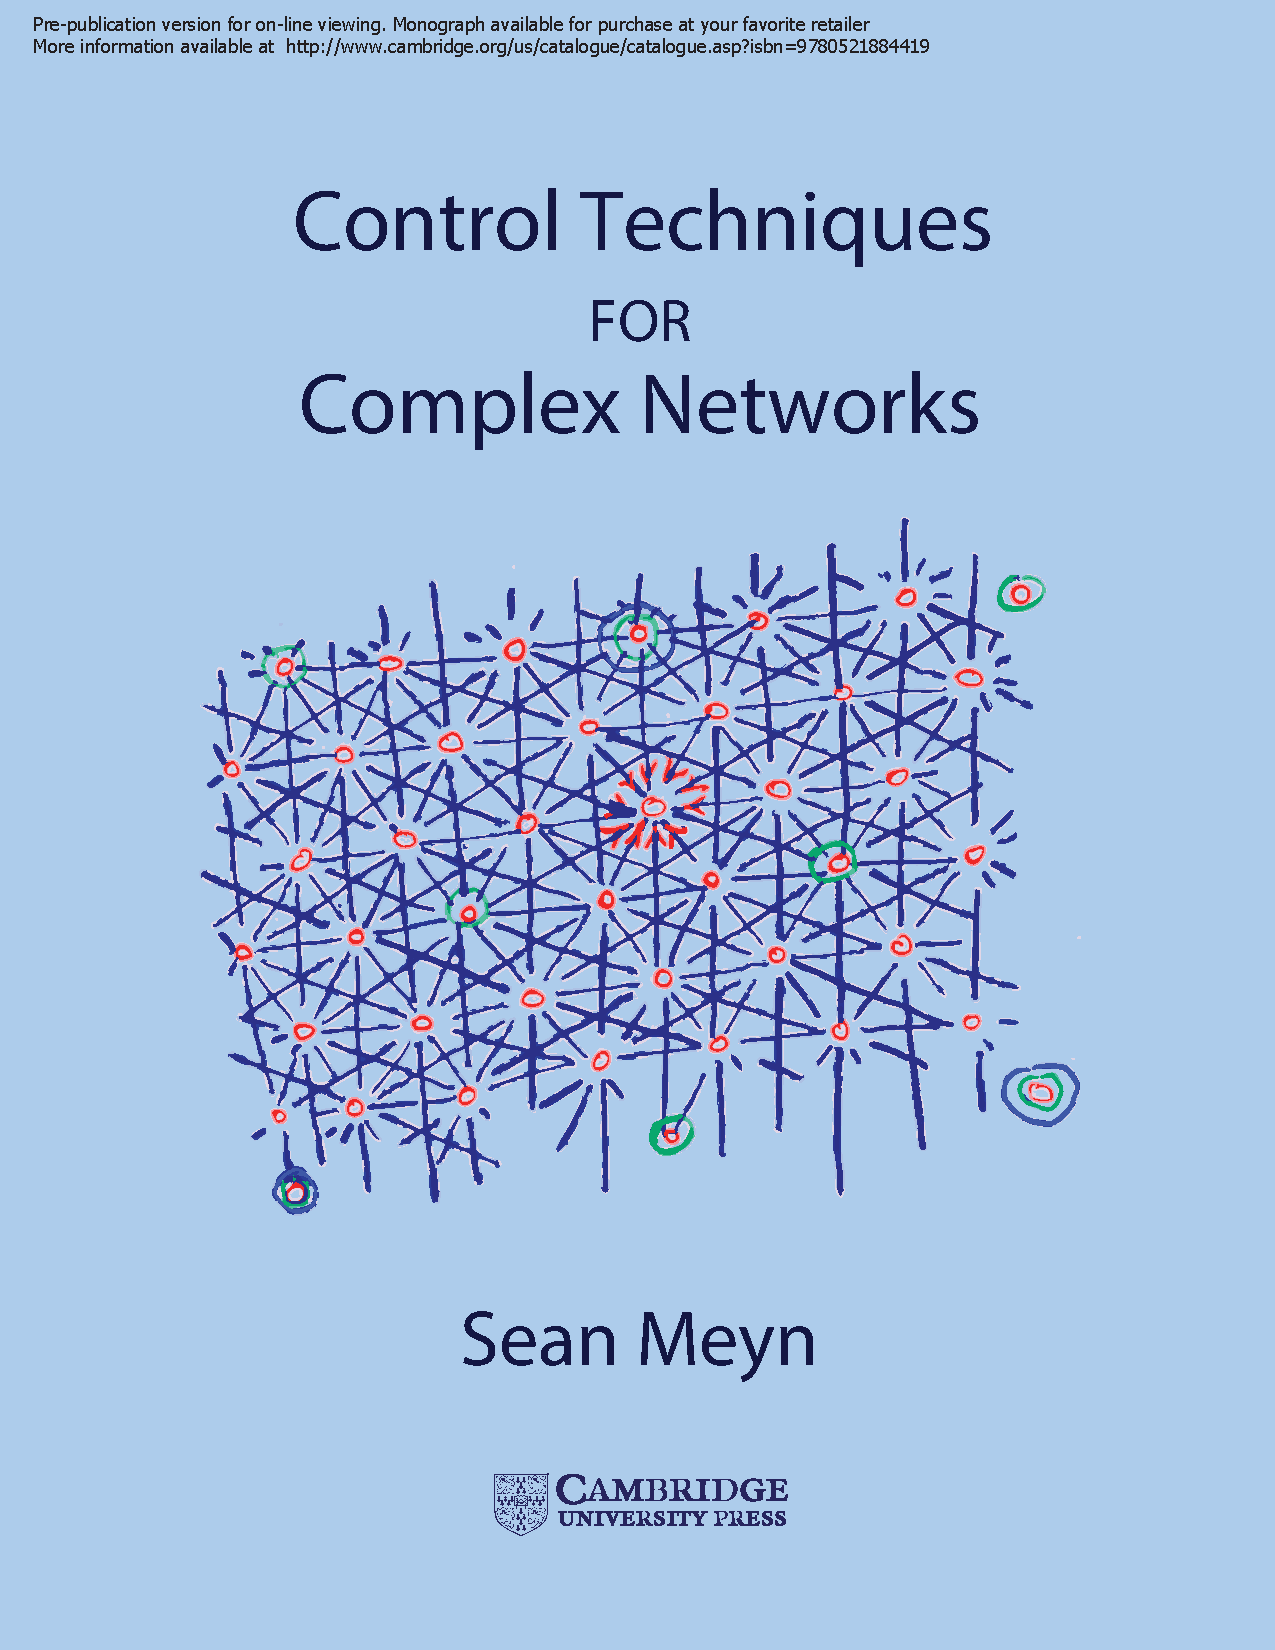
\includegraphics[width=.4\hsize]{CTCN.pdf}} \qquad
%	\href{http://www.meyn.ece.ufl.edu/archive/spm_files/book.html}{
%		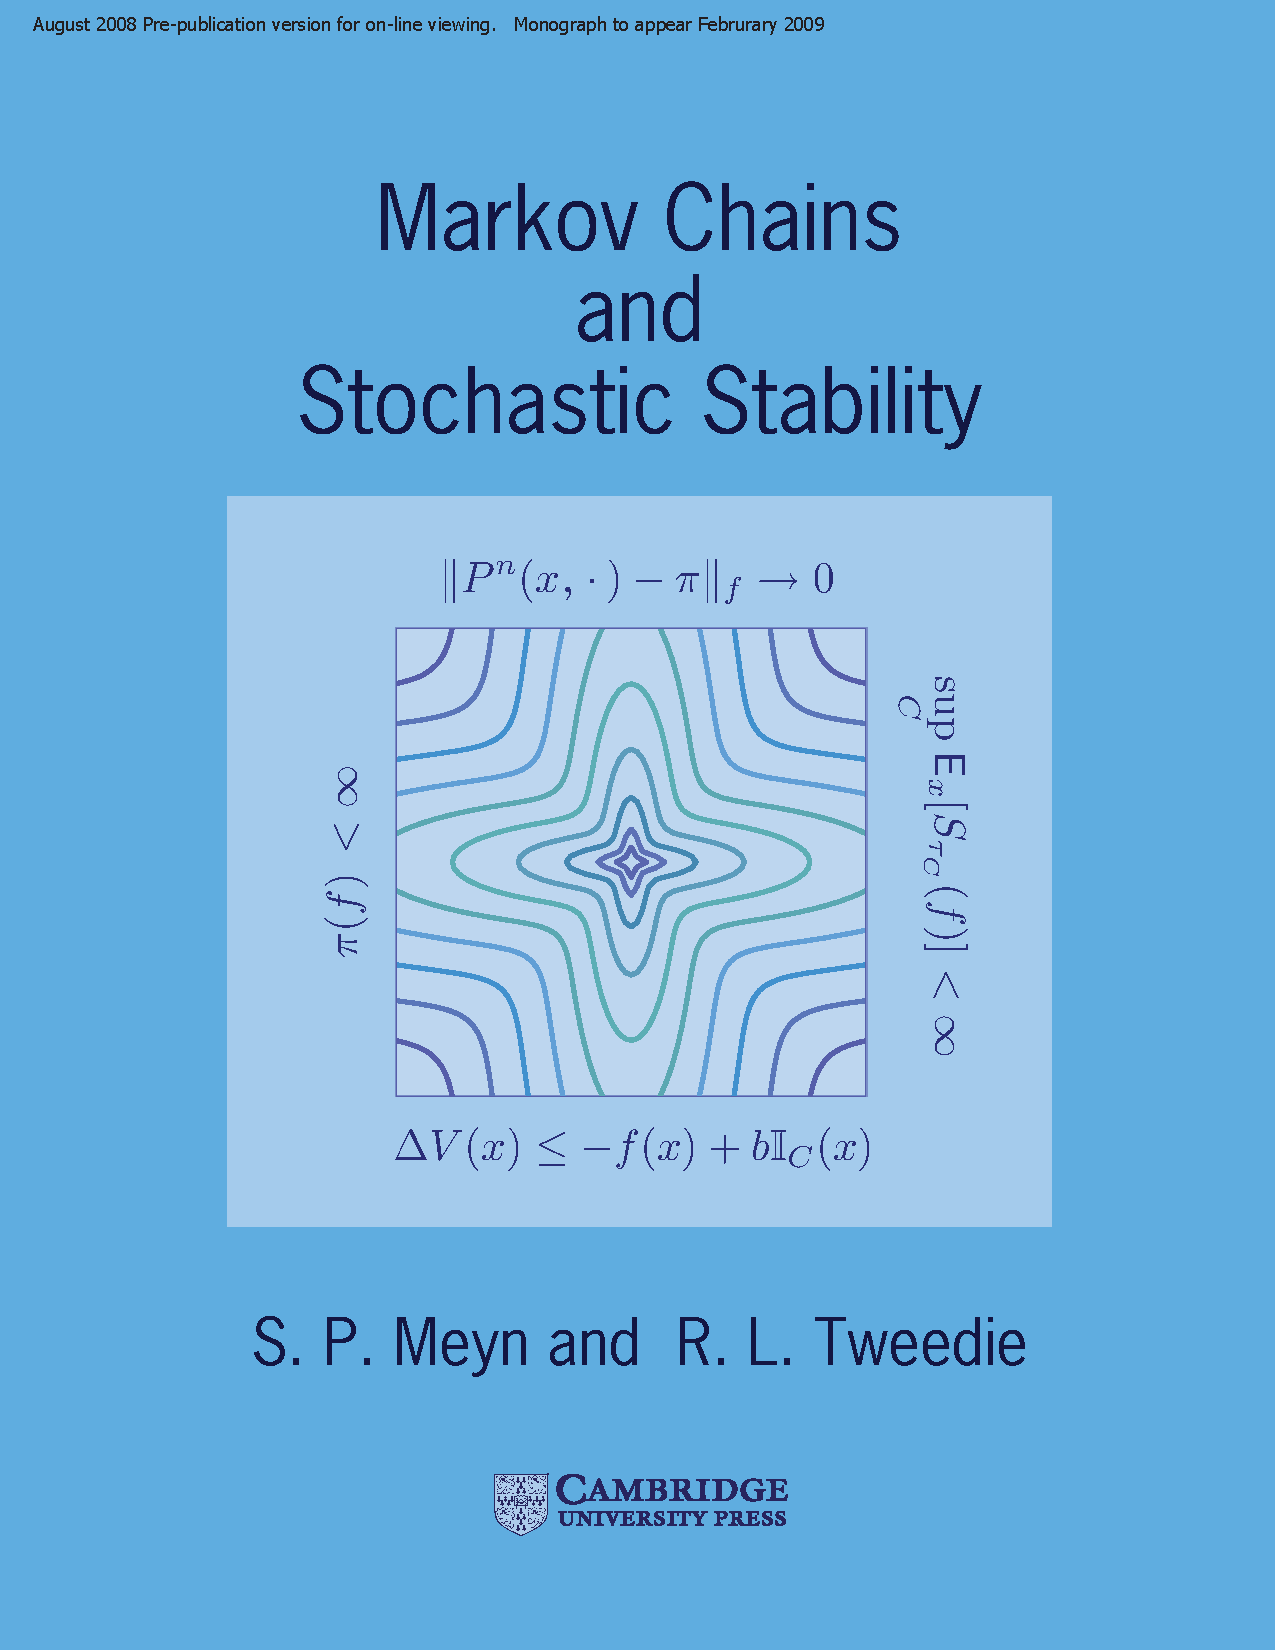
\includegraphics[width=.4\hsize]{CoverMCSS08.pdf}}
%\end{center}
%
%\vfill
%
%\centerline{\Large\bf References}
%
%\vfill
%
%\end{frame}

%\begin{frame}[allowframebreaks]


%\frametitle{Selected References}
%\framesubtitle{Math Background} 


%\setbeamertemplate{bibliography item}{\insertbiblabel}

%\bibliographystyle{alpha}

%\begin{thebibliography}{10}
%\scriptsize
%
%\bibitem{devmey17a}
%A.~M. Devraj and S.~P. Meyn.
%\alert{{{\href{https://arxiv.org/abs/1707.03770}{\em Fastest convergence for Q-learning.}}}}
%{\em ArXiv }, July 2017  (extended version of NIPS 2017).
%
%
%\bibitem{devbusmey18}
%A.~M. Devraj, A.~{Bu{\v s}i{\'c}} and S.~P. Meyn.
%\alert{{{\href{https://arxiv.org/abs/1809.06277}{\em Zap Meets Momentum: Stochastic Approximation Algorithms with Optimal Convergence Rate.}}}}
%{\em ArXiv }, September 2018.
%
%
%\bibitem{benmetpri90}
%A.~Benveniste, M.~M\'etivier, and P.~Priouret.
%\alertb{\em  Adaptive algorithms and stochastic approximations}, volume~22 of
%{\em Applications of Mathematics (New York)}.
%  Springer-Verlag, Berlin, 1990.
%  Translated from the French by Stephen S. Wilson.
%  
%  
%
%\bibitem{bor08a}
%V.~S. Borkar.
%\alertb{\em  Stochastic Approximation: A Dynamical Systems Viewpoint}.
%  {Hindustan Book Agency and Cambridge University Press (jointly)},
%{Delhi, India and Cambridge, UK}, 2008.
%
%
%
%\bibitem{bormey00a}
%V.~S. Borkar and S.~P. Meyn.
% \alertb{\em  The {ODE} method for convergence of stochastic approximation and
%reinforcement learning.}
%  {\em SIAM J. Control Optim.}, 38(2):447--469, 2000. 
%  
%
%
%\bibitem{MT}
%S.~P. Meyn and R.~L. Tweedie.
%\alertb{\em 
%  Markov chains and stochastic stability}.
%  Cambridge University Press, Cambridge, second edition, 2009.
%  Published in the Cambridge Mathematical Library.    
%  
%\bibitem{CTCN}
%S.~P. Meyn.
%\alertb{\em  Control Techniques for Complex Networks}.
%  Cambridge University Press, 2007. 
%  \\
%    \alertc{\it See last chapter on simulation and average-cost TD learning}
%
%%  
%%\setcounter{temp}{\value{enumiv}}
%%
%%  
%%\end{thebibliography}
%%\end{frame}
%%
%%
%%\begin{frame}
%%\frametitle{Selected References}
%%\framesubtitle{Math Background} 
%%%\bibliographystyle{alpha}
%%
%%
%%\setbeamertemplate{bibliography item}{\insertbiblabel}
%%\setcounter{enumiv}{\value{temp}}
%%
%%\begin{thebibliography}{10}
%%\scriptsize
%%
%
%
%
%\bibitem{rup85}
%D.~Ruppert.
%\alertb{\em 
%  A {Newton-Raphson} version of the multivariate {Robbins-Monro}
%procedure.}
%  {\em The Annals of Statistics}, 13(1):236--245, 1985.
%  
%  
%\bibitem{rup88}
%D.~Ruppert.
%\alertb{\em 
%  Efficient estimators from a slowly convergent {Robbins-Monro}
%processes.}
%  Technical Report Tech.~Rept.~No.~781, Cornell University, School of
%Operations Research and Industrial Engineering, Ithaca, NY, 1988.
%
%
%\bibitem{pol90}
%B.~T. Polyak.
% \alertb{\em  A new method of stochastic approximation type.}
%  {\em Avtomatika i telemekhanika (in Russian). translated in Automat.
%	Remote Control, 51 (1991)}, pages 98--107, 1990.
%
%\bibitem{poljud92}
%B.~T. Polyak and A.~B. Juditsky.
%  \alertb{\em Acceleration of stochastic approximation by averaging.}
%  {\em SIAM J. Control Optim.}, 30(4):838--855, 1992.
%  
%
%   \bibitem{pol64}
%B.~T. Polyak.
%\alertb{Some methods of speeding up the convergence of iteration methods.}
%{\em USSR Computational Mathematics and Mathematical Physics},
%4(5):1--17, 1964.
%
%\bibitem{nes83}
%Y.~Nesterov.
%\alertb{A method of solving a convex programming problem with convergence rate ${O} (1/k^2)$.}
%In {\em Soviet Mathematics Doklady}, 1983.
%  
%   
%  
% 
%\bibitem{kontsi04}
%V.~R. Konda and J.~N. Tsitsiklis.
%   \alertb{\em Convergence rate of linear two-time-scale stochastic approximation.}
%  {\em Ann. Appl. Probab.}, 14(2):796--819, 2004.
%
%
%\bibitem{moubac11}
%E.~Moulines and F.~R. Bach.
% \alertb{\em  Non-asymptotic analysis of stochastic approximation algorithms for
%machine learning.}
%  In {\em Advances in Neural Information Processing Systems 24}, pages
%451--459. Curran Associates, Inc., 2011.
%
%
%%\end{thebibliography}
%%\end{frame}
%
%%
%% \begin{frame}
%%\frametitle{Selected References}
%%\framesubtitle{Reinforcement Learning} 
%%\bibliographystyle{alpha}
%%
%%\begin{thebibliography}{10}
%
%%\scriptsize
%\bibitem{sze10}
%C.~Szepesv{\'a}ri.
%  \alertb{\em  Algorithms for Reinforcement Learning}.
%  Synthesis Lectures on Artificial Intelligence and Machine Learning.
%Morgan {\&} Claypool Publishers, 2010.
%
%
%\bibitem{watday92a}
%C.~J. C.~H. Watkins and P.~Dayan.
%\alertb{\em 
%  {$Q$}-learning.}
%  {\em Machine Learning}, 8(3-4):279--292, 1992. 
%
%\bibitem{sut88}
%R.~S. Sutton.\alertb{\em 
%  Learning to predict by the methods of temporal differences.}
%  {\em Mach. Learn.}, 3(1):9--44, 1988.
% 
%  
%  
%
%\bibitem{tsiroy97a}
%J.~N. Tsitsiklis and B.~Van~Roy.
% \alertb{\em  An analysis of temporal-difference learning with function
%approximation.}
%  {\em IEEE Trans. Automat. Control}, 42(5):674--690, 1997.
%
%
%
%\bibitem{sze97}
%C.~Szepesv{\'a}ri.
% \alertb{\em  The asymptotic convergence-rate of {Q-learning}.}
%  In {\em Proceedings of the 10th Internat.\ Conf.\ on Neural Info.\ Proc.\ Systems}, pages 1064--1070. MIT Press, 1997.
%
%
%
% 
%\bibitem{azamunghakap11}
%M.~G. Azar, R.~Munos, M.~Ghavamzadeh, and H.~Kappen.
%  \alertb{\em Speedy {Q}-learning.}
%  In {\em Advances in Neural Information Processing Systems}, 2011.
%  
%
%\bibitem{eveman03}
%E.~Even-Dar and Y.~Mansour.
%\alertb{\em Learning rates for {Q}-learning.}
%  {\em Journal of Machine Learning Research}, 5(Dec):1--25, 2003.
% 
% 
% 
% \bibitem{huachemehmeysur11}
%D.~Huang, W.~Chen, P.~Mehta, S.~Meyn, and A.~Surana.
%\alertb{\em  Feature selection for neuro-dynamic programming.}
%  In F.~Lewis, editor, {\em Reinforcement Learning and Approximate
%  Dynamic Programming for Feedback Control}. Wiley, 2011.
%
% 
%  
%% 
%%\end{thebibliography}
%%\end{frame}
%%
%% \begin{frame}
%%\frametitle{Selected References}
%%\framesubtitle{Reinforcement Learning} 
%%\bibliographystyle{alpha}
%%
%%\begin{thebibliography}{10}
%%\scriptsize
%
% 
%
%  
%
%
%\bibitem{tsiroy99}
%J.~N. Tsitsiklis and B.~Van~Roy.
%  \alertb{\em Optimal stopping of {M}arkov processes: {H}ilbert space theory,
%approximation algorithms, and an application to pricing high-dimensional
%financial derivatives.}
%  {\em IEEE Trans. Automat. Control}, 44(10):1840--1851, 1999.
%  
%  
%\bibitem{choroy06}
%D.~Choi and B.~Van~Roy.
%\alertb{\em A generalized {Kalman} filter for fixed point approximation and
%efficient temporal-difference learning.}
%  {\em Discrete Event Dynamic Systems: Theory and Applications},
%16(2):207--239, 2006.
%
%   
%
%
%\bibitem{brabar96}
%S.~J. Bradtke and A.~G. Barto.
% \alertb{\em  Linear least-squares algorithms for temporal difference learning.}
%  {\em Mach. Learn.}, 22(1-3):33--57, 1996.
%
%  
%\bibitem{boy02}
%J.~A. Boyan.
%\alertb{\em Technical update: Least-squares temporal difference learning.}
%  {\em Mach. Learn.}, 49(2-3):233--246, 2002.
%
%
%
%\bibitem{nedber03a}
%A.~Nedic and D.~Bertsekas.
%\alertb{\em Least squares policy evaluation algorithms with linear function
%approximation.}
%  {\em Discrete Event Dyn.\ Systems: Theory and Appl.},
%13(1-2):79--110, 2003.
%
% 
%
%\bibitem{mehmey09a}
%P.~G. Mehta and S.~P. Meyn.
%\alertb{\em Q-learning and {Pontryagin's} minimum principle.}
%  In {\em {IEEE} Conference on Decision and Control}, pages 3598--3605,
%Dec. 2009.
% 
%  
%\end{thebibliography}
%\end{frame}


 \end{document}
%\begin{frame}
%\frametitle{Finite-$n$ bounds} 
%
%\begin{block}{Watkin's Q Learning (Szepesv\'ari 1998)}
%
%\begin{equation*}
%\begin{aligned}
%|\theta - \theta^*| & \leq \frac{B}{t^{R(1-\beta)}}
%\\
%|\theta - \theta^*| & \leq B \sqrt{\frac{\log \log t}{t}}
%\end{aligned}
%\end{equation*}
%
%\end{block}
%
%\begin{block}{Speedy Q Learning (Azar et.\ al.)}
%
%\begin{equation*}
%\begin{aligned}
%|\theta - \theta^*| & \leq \frac{B}{t^{R(1-\beta)}}
%\\
%|\theta - \theta^*| & \leq B \sqrt{\frac{\log \log t}{t}}
%\end{aligned}
%\end{equation*}
%
%\end{block}
%
%\end{frame}

 
\section{Appendix:  Quick RL and MDP Tutorial}


%\ad{Find figures!}
\begin{framesection}

\centering

\Ebox{.85}{Fig2_mystery.pdf}

\vfill
\Large\bf  Reinforcement Learning
\\
and Stochastic Approximation

\end{framesection}
\subsection{RL \&\ SA}

\subsection{MDP Theory}

\begin{frame}
\frametitle{Stochastic Optimal Control} 

\begin{block}{MDP Model}
$\bfmX$ is a stationary controlled Markov chain, with input $\bfmU$ 
\begin{itemize}
\item For all states $x$ and sets $A$,
\vspace{-0.1in}
\[
\Prob\{X_{n+1}\in A \mid X_{n}=x,\ U_{n}=u, \text{\small and prior history} \} = P_u(x,A)
\]
\item
\vspace{-0.1in}
$c\colon\state\times\U\to \Re$ is a cost function

\item
$\beta<1$ a discount factor
\end{itemize}
\end{block}

\pause


\begin{alertblock}{Q function:}
\vspace{-0.1in}
\[
Q^*(x, u) = \alert{\min_\bfmU} \sum_{n=0}^\infty \beta^n \Expect[c(X_{n},U_{n}) \mid X(0) =x, U(0) = u]
\]
\end{alertblock}


\pause

\begin{alertblock}{Bellman equation:}
\vspace{-0.1in}
\[
Q^*(x, u)=
c(x,u) + \beta \Expect \big [ \displaystyle\min_{u'}  Q^*(X_{n+1}, u') \mid X_{n} =x,\ U_{n}=u \big ]
\]
\end{alertblock}

\end{frame}

%\subsection{TD-Learning}
%\begin{frame}
%\frametitle{Optimal Control \qquad \small TD-Learning} 
%Approximate value function obtained for a fixed policy:
%\[
%h^\theta(x)\approx 
%h(x) =   \sum_{t=0}^\infty \beta^t \Expect[c(X_{n},U_{n}) \mid X(0) =x]
%\]
%\vspace{-.5cm}
%Two flavors:
%\begin{itemize}
%\item  $\displaystyle \min_\theta \Expect\bigl[ \bigl( h(X) - h^\theta(X) \bigr)^2\bigr]$.  
%\pause  Search for solution to
%\[
%0= \Expect\bigl[ \alert{\bigl( h(X) - h^\theta(X) \bigr) \nabla_\theta h^\theta(X) }\bigr]
%\]
%\pause
%\item  
%%\hfill $0= \Expect[c(X_{n},U_{n}) + \beta h(X_{n+1}) - h(X_{n}) \mid X_{n}=x]  $
%Galerkin relaxation of Bellman equation:
%\\
%For a stationary vector-valued sequence $\{\alertd{\elig_n}\}$,
%\[
%0= \Expect\bigl[  \alert{\bigl(  c(X_{n},U_{n}) + \beta h^\theta(X_{n+1}) - h^\theta(X_{n})  \bigr) \alertd{\elig_n }}
%\bigr]
%\]
%\end{itemize}
% \vfill
%% \alertc{\textit{$Q$-learning:  another Galerkin relaxation}}
%\end{frame}


\begin{frame}
\frametitle{$Q$-learning and Galerkin Relaxation}
  
\begin{minipage}[t][10cm][t]{\textwidth}

\uncover<1->{
\begin{alertblock}{\alertd{Dynamic programming}}
Find function $Q^*$ that solves
\[
\Expect\bigl[ 
c(X_{n},U_{n}) +\beta  \uQ^*(X_{n+1})  -  Q^*(X_{n},U_{n})  \mid {\cal F}_n \bigr] =0
\]
\end{alertblock}
}

\uncover<2->{ \vspace{1em}
\begin{alertblock}{Q-Learning}
Given \{$Q^\theta: \theta \in \Re^d$\}, find $\theta^*$ that solves
\[
\Expect\bigl[  \alertb{\bigl(  c(X_{n},U_{n}) + \beta \uQ^{\theta^*}((X_{n+1}) - Q^{\theta^*}((X_{n},U_{n})  \bigr) }  {\color{violet}{\elig_n}} 
\bigr] = 0
\]
The family $\{ Q^\theta\}$ and ``\textit{\color{violet} eligibility vectors}" $ \{  {\color{violet}\zeta_n} \}$ are part of algorithm design. 
\end{alertblock}
}
\end{minipage}

\end{frame}


% \ad Let's look at the linear case:
\begin{frame}
\frametitle{$Q$-learning and Stochastic Approximation}

\begin{minipage}[t][10cm][t]{\textwidth}

\vspace{-0.25in}
\uncover<1->{
\begin{alertblock}{\alertc{ $Q$-learning:} \color{black}{$Q^\theta(x,u) = \theta^{\transpose} \psi(x,u) \qquad \quad \theta \in \Re^d\,, \,\,\,\, \psi: \state \times \U \to \Re^d$}}

Find $\theta^*$ such that:
\[
\Expect\bigl[  \alertb{\bigl(  c(X_{n},U_{n}) + \beta \uQ^{\theta^*}((X_{n+1}) - Q^{\theta^*}((X_{n},U_{n})  \bigr) }  {\color{violet}{\elig_n}} 
\bigr] = 0
\]
\hfill 
Example:  $ {\color{violet}{\zeta_n} = \nabla_\theta Q^\theta(X_{n}, U_{n}) = \psi(X_{n},U_{n})}$
\end{alertblock}
}


\uncover<2->{
\begin{block}{$Q$-learning and SA}
Root finding problem: \qquad
$
\barf(\theta^*) = \bfmA (\theta^*) \theta^* - \bfmb = 0
$
}


\uncover<3->{
\[
\begin{aligned}
\bfmA (\theta) &= \Expect\bigl[   {\color{violet}{\zeta_n}}   { \bigl[\beta \psi(X_{n+1}, \alertd{\phi^\theta(X_{n+1})}) 
-  \psi(X_{n},U_{n})    
\bigr]^\transpose }\,\, \bigr]
\\
\bfmb & \eqdef \Expect\big[ {\color{violet}{\zeta_n}} c(X_n, U_n) \big]
\\
\alertd{\phi^\theta(x)} & \eqdef \argmin_u Q^\theta(x, u)
\end{aligned}
\]
\end{block}
}
\end{minipage}
\end{frame}



\begin{frame}
\frametitle{Watkins' $Q$-learning}

\begin{minipage}[t][10cm][t]{\textwidth}
\uncover<6->{
\vspace{-0.1in}
\begin{center}
\framebox{
\alertc{
\Large  Big Question:  \it
Can we Zap Q-Learning?
}
}
\end{center}
\vspace{-0.2in}
}


\uncover<1->{
\[
\Expect\bigl[  \alert{  \bigl(  c(X_{n},U_{n}) + \beta \uQ^{\theta^*}(X_{n+1}) - Q^{\theta^*}(X_{n},U_{n})  \bigr)   {\color{violet}{ \zeta_n}} }
\bigr] = 0
\]
}

\vspace{-0.05in} 

\uncover<2->{
\vspace{-1em}
\begin{block}{Watkin's algorithm is Stochastic Approximation}

The family $\{ Q^\theta\}$ and \textit{eligibility vectors} $ \{  \color{violet}{ \zeta_n} \}$ in this  design:
\begin{itemize} 
\item 
Linearly parameterized family of functions: $Q^\theta (x,u) = \theta^\transpose \psi(x,u)$
\item 
${\color{violet}{\elig_n}} \equiv \psi(X_{n},U_{n})$ % \qquad \textit{and}
\item  $\psi_i(x,u) = \ind \{x=x^i, u=u^i\}$ \qquad (complete basis)
\end{itemize}
\end{block}
}

\only<3>{ 
\begin{alertblock}{Algorithm:}
\vspace{-0.1in}
\[
\theta_{n+1} = \theta_n + \alpha_{n+1} \alert{  \bigl(  c(X_{n},U_{n}) + \beta \uQ^{\theta^*}(X_{n+1}) - Q^{\theta^*}(X_{n},U_{n})  \bigr)   {\color{violet}{ \zeta_n}} }
\]
%\rightline{\alert{[Devraj \& M, 2017]}}
\end{alertblock}}

\only<4>{ 
\begin{alertblock}{Converges, but has infinite asymptotic variance if $\beta > \half$:}
\vspace{-0.1in}
\[
 \lambda_{\max} \big (\bfmA(\theta^*) \big ) > - \half
\]
\rightline{\alert{[Devraj \& M, 2017]}}
\end{alertblock}}
\only<5-6>{
\begin{alertblock}{Convergence rate for $\beta > \half$:}
\vspace{-0.1in}
\[
\clO(1/n^{1-\beta})
\]
\rightline{\alert{[Devraj \& M, 2017]}}
\end{alertblock}}
\end{minipage}
\end{frame}


\begin{framesection}

\Ebox{1}{Zapdos_6State_BEPlot_Beta099-1.pdf} 

\vfill

\centerline{\Large\bf  Zap Q-Learning} 

\end{framesection}
 
 \end{document}
 
 
 
 


